\documentclass[12pt, a4paper]{article}
\usepackage[english]{babel}
\usepackage[utf8]{inputenc}
\usepackage[T1]{fontenc}
\usepackage{amsmath}
\usepackage{amssymb}
\usepackage{amsthm}
\usepackage{hyperref}
\usepackage{cleveref}
\usepackage{xcolor}
\usepackage{algorithm}
\usepackage{algpseudocode}
\usepackage{graphicx}
\usepackage{subfigure}

\newtheorem{definition}{Definition}
\newtheorem{example}{Example}
\newtheorem{theorem}{Theorem}
\newtheorem{lemma}{Lemma}

\begin{document}
\title{When two-point correlation function fails to describe a structure...}
\author{Biba and Boba}
\maketitle

\section{Introduction}
AAA BBB

\section{All the math}
\subsection{Definitions}
Suppose $A$ is some region in a Euclidean space $\mathbb{R}^n$. Let
$A_1, A_2, \dots, A_N$ be subsets of $A$ so that
\begin{align*}
  \cup_{i=1}^N A_i &= A \\
  A_i \cap A_j &= \emptyset, \ i \ne j
\end{align*}
It is said that the point $x$ is in the phase $i$ if $x \in A_i$.

Define a set of characteristic functions $\chi_i(x)$ as follows:
\begin{equation*}
  \chi_i(x) = \left\{
  \begin{array}{ll}
    1 & \quad \text{if $x \in A_i$} \\
    0 & \quad \text{otherwise}
  \end{array}
  \right.
\end{equation*}

The two-point correlation function
$S_2^{(i)}: \mathbb{R}^n \rightarrow \mathbb{R}$ for homogeneous media can
defined in the terms of $\chi$:
\begin{equation}
  S_2^{(i)}(r) = \langle \chi_i(x) \chi_i(x+r) \rangle
  \label{eq:s2}
\end{equation}
where $\langle \dots \rangle$ means ensemble average. Its meaning is given in
the following definition:
\begin{definition}
  The two-point correlation function $S_2^{(i)}(r)$ is a probability that a
  line segment $r$ thrown randomly into $A$ has its both ends in the phase $i$.
  \label{def:s2}
\end{definition}

Two-phase media in which the region $A$ is subdivided in two adjacent phases
(usually called ``void'' and ``solid'') are of special interest for practical
applications. In this case function $S_2^{(1)}$ and $S_2^{(0)}$ has a linear
dependency \cite{Torquato_book}:
\begin{equation*}
  S_2^{(1)}(r) = S_2^{(0)}(r) + 1 - 2S_2^{(0)}(0)
\end{equation*}
In our paper we will stick to $S_2^{(1)}$ function for simplicity.

In practice the region $A$ is a $n$-dimensional array, vectors $r$ and $x$ can
have integer coefficients and $x \in A^{(1)}$ is equivalent to $A[x] = 1$
(element at the index $x$ is equal to $1$). The two-point correlation function
is then computed using fast Fourier transform.

A problem of reconstruction of $A$, i.e. properly finding its subset $A_1$, from
its two-point correlation function is often arises in porous materials
science. In this paper we approach the problem of reconstruction having a
so-called full correlation map of $A$, i.e. the values $S_2^{(1)}(x)$ for
$x \in (1 \dots 2D_1-1)\times(1 \dots 2D_2-1)\times\dots$ where
$D_1, D_2, \dots$ are dimensions of the array $A$. Here multiplication by two
and subtraction of one means that we consider two-point function calculated with
zero padding, described in the next subsection.

\subsection{Boundary conditions}
The two-point correlation function can be calculated with periodic boundary
conditions and zero padding depending on whether a line segment in
\cref{def:s2} is allowed to cross the boundary of array or not. If it is allowed
to do so, its coordinates are ``wrapped'' around the boundary, i.e. taken
$\mod D$, $D = (D_1, D_2, \dots)$ (\cref{fig:s2-computation}).
\begin{figure*}[tp]
  \centering
  \subfigure[Periodic boundary conditions]{
    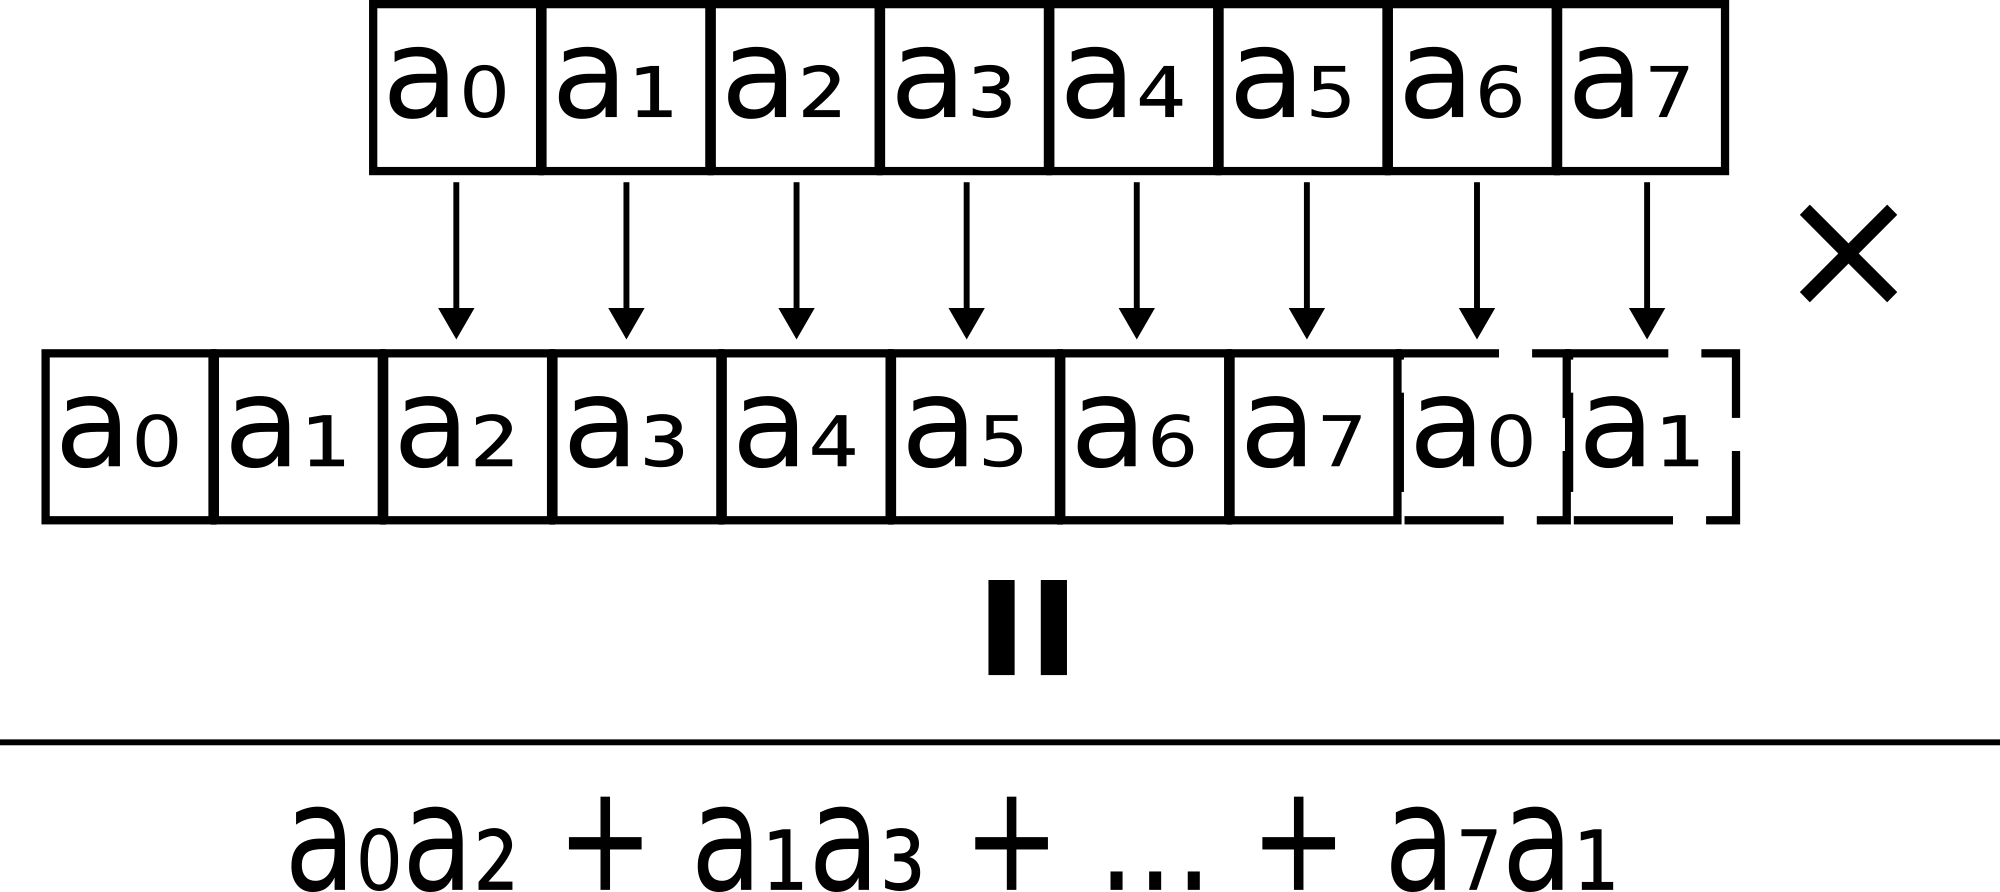
\includegraphics[width=0.4\linewidth]{images/periodic.png}
    \label{fig:s2-periodic}}
  \hfill
  \subfigure[Zero padding]{
    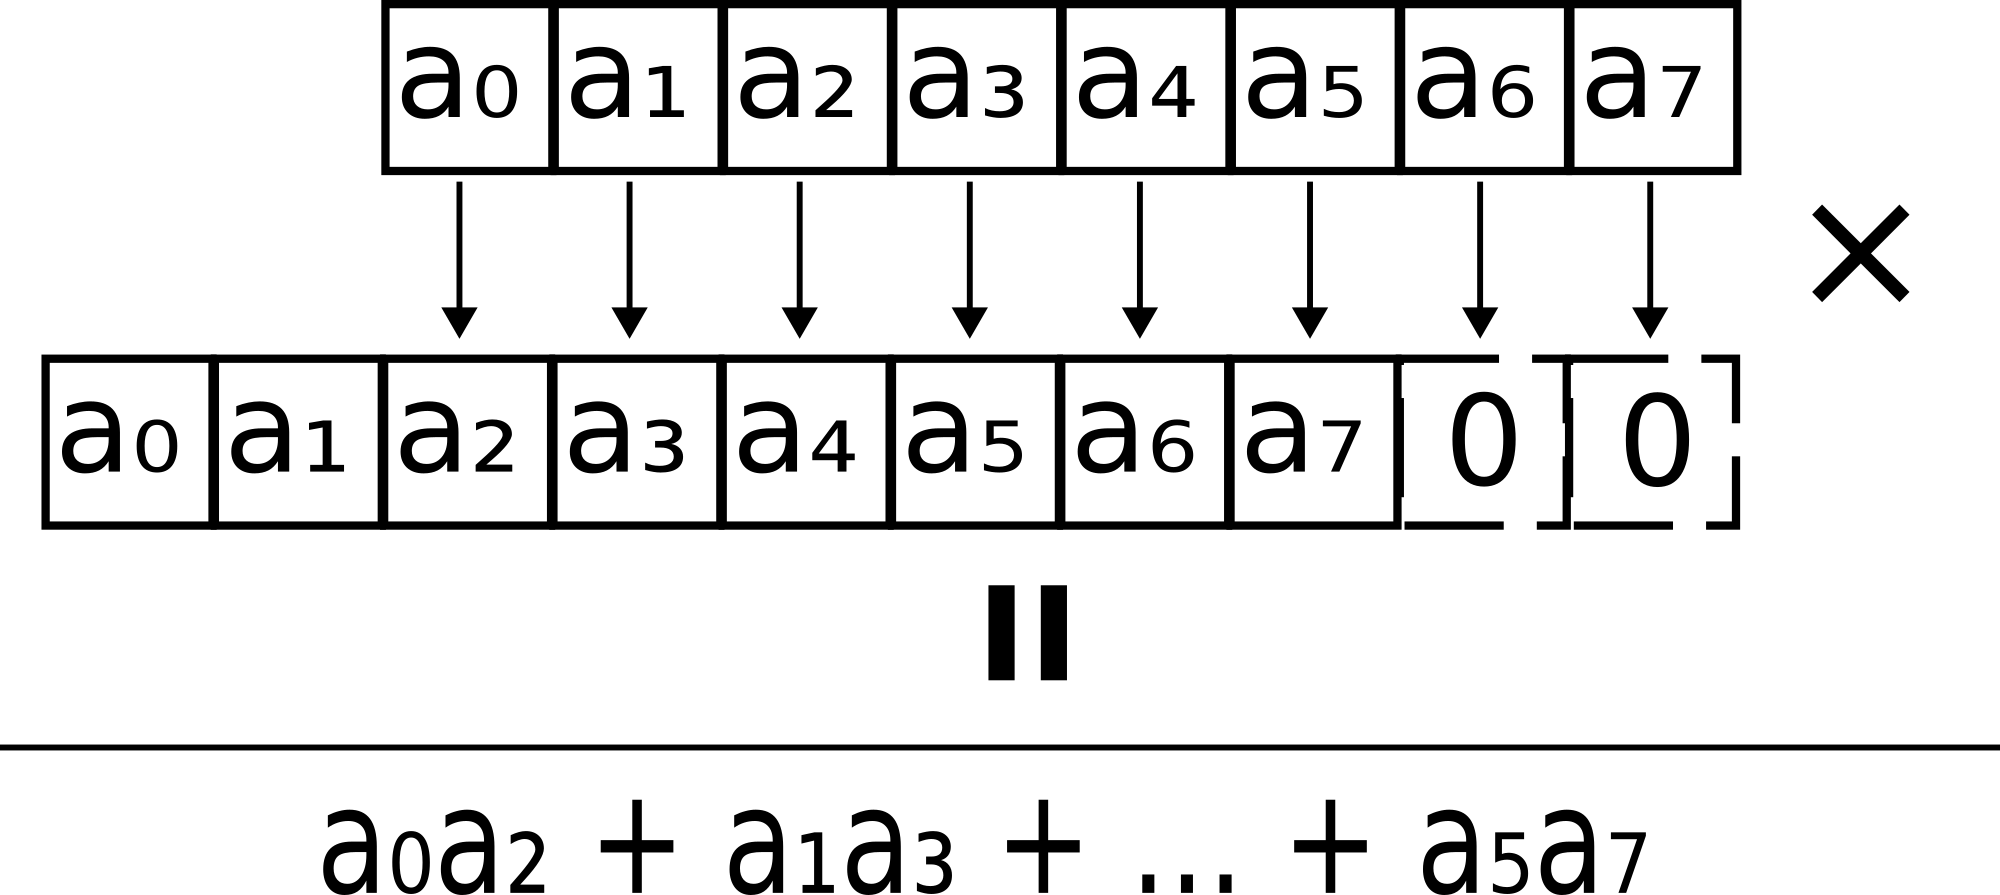
\includegraphics[width=0.4\linewidth]{images/zeros.png}
    \label{fig:s2-zeros}}
  \caption[]{Computation of the two-point correlation function at the point $2$
    for one-dimensional sequence of length 8.}
  \label{fig:s2-computation}
\end{figure*}

In this paper we will primarily discuss the two-point function calculated with
zero padding.

\subsection{Collisions in the two-point function for sequences of 0's and 1's}
When reconstructing a two-phase porous medium from its correlation function, it
is important to know to what extent a reconstruction will resemble the original
image. Consider the following definition:
\begin{definition}
  Arrays $A$ and $B$ of the same dimensionality have a collision in the
  two-point correlation function if they have the same values of this function
  in all points of its definition, but $A \ne B$.
\end{definition}

Turns out that every array $A$ has a collision of two specific forms, which we
will discuss after describing a mathematical framework which will help us in the
analysis.

\begin{definition}
  A Z-transform of a sequence $\{a_0, a_1, \dots, a_n\}$ is a polynomial
  $\sum_{i=0}^n a_i z^{-i}$.
\end{definition}
Z-transform is much like the discrete Fourier transform, particulary it has the
same convolution theorem:
\begin{theorem}
  If $g(z)$ and $h(z)$ are images of sequences $a$ and $b$ under Z-transform,
  then $g(z)h(z) = f(z)$ where $f(z)$ is an image of $a*b$ under Z-transform
  and $a*b$ is a discrete convolution of $a$ and $b$:
  \begin{equation*}
    (a*b)_k = \sum_{i=0}^{n} a_i b_{k-i}
  \end{equation*}
  \label{th:conv}
\end{theorem}
In the case of one-dimensional two-phase porous media $a$ the definition
\ref{eq:s2} can be rewritten as follows
\begin{equation*}
  S_2(r) = \frac{\sum_{i}a_ia_{i+r}}{N(r)}
\end{equation*}
where $N(r)$ is a normalization factor which does not depend on $a$ and can be
omitted for simplicity. The numerator is a discrete autocorrelation which is
equal to a convolution of $a$ with ``reversed'' $a$, i.e. $i$-th element of $a$
becomes $-i$-th element of a reversed sequence. Let $f(z)$ be an image of $a$
under Z-transform. Then an image $s_2(z)$ of the sum above can be calculated
using \cref{th:conv}.
\begin{equation}
  s_2(z) = f(z)f(z^{-1})
  \label{eq:s2z}
\end{equation}
Making a substitution $t^{-1} = z + z^{-1}$ and inverting $s_2(t)$ we will get a
sequence $S_2(r) = (S_2(0), S_2(1), S_2(2), \dots)$ up to a normalization by
$N(r)$. The meaning of this sequence is a number of positive elements in $a$
distanced by $r$.
\begin{example}
  Let $a$ be a sequence $(1, 0, 1, 0, 0, 1)$. Its Z-transform is
  $f(z) = 1 + z^{-2} + z^{-5}$.
  \begin{align*}
    s_2(z) &= f(z)f(z^{-1}) \\
    &= (1 + z^{-2} + z^{-5})(1 + z^2 + z^5) \\
    &= (1 + z^2 + z^5) + (z^{-2} + 1 + z^3) + (z^{-5} + z^{-3} + 1) \\
    &= 3 + (z^2 + z^{-2}) + (z^3 + z^{-3}) + (z^5 + z^{-5})
  \end{align*}
  Thus, we have $s(t) = 3 + t^{-2} + t^{-3} + t^{-5}$. Inverting, we obtain a
  sequence $(3, 0, 1, 1, 0, 1)$, which means that $a$ has three elements in
  phase $1$, zero adjacent elements in phase $1$, one pair which is distanced by
  2 (elements with indices 0 and 2), one pair distanced by 3 (indices 2 and 5)
  and one pair distanced by 5 (indices 0 and 5).
\end{example}

By looking at \cref{eq:s2z} it becomes clear that the following two
substitutions, designated $S_k$ and $R$, do not change $s_2(z)$ and hence, the
two-point correlation function:
\begin{equation}
  \begin{aligned}
    R&: f(z) \rightarrow f(z^{-1}) \\
    S_k&: f(z) \rightarrow z^{-k}f(z)
  \end{aligned}
  \label{eq:group-elts}
\end{equation}
The set
\begin{equation}
  G = \{R, S_0, S_1, S_{-1}, \dots \}
  \label{eq:group}
\end{equation}
and a binary operation $\circ$ (composition) form a group of transforms of $a$
which do not change the two-point function. Its neutral element is $S_0$ and the
associativity and invertibility are trivial to prove.

The transform $R$ means a reversion of a sequence, i.e. writing it ``the other
way around''. The transform $S_k$ means shifting a sequence to the right by $k$
elements. These are trivial transforms which are already present in the
literature. It is clear that any two sequences $a$ and $Ta$, $T \in G$ form a
collision, so if we search for collisions, it is important to ``discard''
trivial collisions like that.

To find non-trivial collisions we firstly introduce a change of variables
$x = z^{-1}$ which is justified by a symmetry of \cref{eq:s2z}. Secondly we
introduce a notion of a reciprocal polynomial and palindrome polynomials.
\begin{definition}
  A reciprocal polynomial of $f(x)$ is a polynomial $x^{\deg f}f(x^{-1})$. A
  polynomial is called a palindrome if it is equal to its reciprocal.
\end{definition}
Examples of palindrome polynomials include $x$, $x + 1$, $x^2 - 2x + 1$, but not
$x^3+x+1$.

Now a mechanism for finding collisions for a two-phase sequence $a$ is
described. Suppose $f(x)$ is a Z-transform of $a$ with aforementioned change of
variables. Its coefficients is therefore belong to a set $\{0, 1\}$ with the
leading and the free coefficients being equal to $1$. The assumption on the free
coefficient is taken without a loss of generality. Indeed, if the free
coefficient is zero, then a monomial $x^n$ divides $f$, and the following
construction can be applied to $\hat{f} = f / x^n$ which has the same
correlation function as $f$.

A reciprocal polynomial of $f(x)$ has the same degree as $f$. Suppose $f$
factors into $M$ different factors in $\mathbb{Z}[x]$:
\begin{equation*}
  f(x) = \prod_{i=1}^M f_i(x)
\end{equation*}
The image of the two-point function is then
\begin{equation*}
  s(x) = f(x)f(x^{-1}) = \prod_{i=1}^M f_i(x) \prod_{i=1}^M f_i(x^{-1})
\end{equation*}
Let now select $1 \le L < M$ non-palindrome factors
$f_{r_1}, f_{r_2}, \dots, f_{r_L}$ of $f$ and replace them with their
reciprocals. Obviously, the resulting correlation function won't change:
\begin{equation*}
  s(x) = \underbrace{\prod_{i=1}^L x^{\deg f_{r_i}} f_{r_i}(x^{-1}) \prod_{i=1}^{M-L} f_{o_i}(x)}_{\tilde{f}(x)}
  \underbrace{\prod_{i=1}^L x^{-\deg f_{r_i}} f_{r_i}(x) \prod_{i=1}^{M-L} f_{o_i}(x^{-1})}_{\tilde{f}(x^{-1})}
\end{equation*}
where $o_1, o_2, \dots, o_{M-L}$ run through indices of original (not replaced)
factors. Now recombining factors into $\tilde{f}(x)$ and $\tilde{f}(x^{-1})$ we
obtain a polynomial $\tilde{f}$ with the same degree as $f$ and $f(0) = \tilde{f}(0)$.
Now note that with this additional demand on the free coefficient, we can
restrict the group of transforms \cref{eq:group} to a subgroup $\{S_0, R\}$
because a non-zero shift will change the degree of $f$ which is not allowed. We
have two possible outcomes regarding $\tilde{f}$:
\begin{itemize}
\item Only at most one factor in $f_{r_1}, \dots, f_{r_L}$ is not a
  palindrome. This gives us $\tilde{f}(x) = f(x^{-1})$ which is a trivial
  collision.
\item At least two factors in $f_{r_1}, \dots, f_{r_L}$ are not palindromes. In
  this case $\tilde{f} \ne f$ and cannot be obtained from $f$ using transforms
  in the subgroup $\{S_0, R\}$.
\end{itemize}

\textcolor{blue}{It is trivial to prove that $\sum_if_i^2 = \sum_i\tilde{f}_i^2$
  where $f_i$ and $\tilde{f}_i$ are coefficients of $f$ and $\tilde{f}$
  respectively. Indeed, $f$ and $\tilde{f}$ have the same correlation function,
  and evaluating $S_2(0)$ gives us the desired result. We also make a conjecture
  that $f$ and $\tilde{f}$ have the same number of non-zero coefficients and
  thus, all coefficients of $\tilde{f}$ are either $0$ or $1$.}
\textcolor{red}{It's better to find a proof for this claim, but no bad things
  can happen, if we cannot.}

Now it must be clear how to find all the non-trivial collisions of $f$. To do so
one must follow \cref{alg:collisions}.
\begin{algorithm}
  \caption{An algorithm for finding non-trivial collisions of $f$ in the
    two-point correlation function.}
  \label{alg:collisions}
  \begin{algorithmic}[1]
    \Procedure{$Collisions$}{$f$}
    \State $fs \gets factor(f \in \mathbb{Z}[x])$
    \State $ps \gets filter(isPalindrome, fs)$
    \State $nps \gets fs \setminus ps$
    \If{$length(nps) \le 1$}
    \State \textbf{return} $f$ has only trivial collisions
    \EndIf
    \State $(np:nps') \gets nps$
    \State $f' \gets np \times \prod ps$
    \State $cs \gets \text{all possible combinations of $nps'$ or reciprocals}$
    \State \textbf{return} $map(f'\times, cs)$
    \EndProcedure
  \end{algorithmic}
\end{algorithm}
Here ``all possible combinations of $nps'$ or reciprocals'' needs
clarification. For each polynomial in $nps'$ either that polynomial or its
reciprocal is taken in a combination of factors $c$ and $cs$ is a list of all
possible $c$'s. If $f$ has $L$ non-palindrome factors as before, we get
$2^{L-1}$ polynomials (including $f$) which have the same two-point function as
$f$.

It is clear to see, that non-trivial collisions of $f$ found using
\cref{alg:collisions} are indeed all non-trivial collisions of $f$, because the
ring $\mathbb{Z}[x, x^{-1}]$ of images of the two-point function under
Z-transform is a UFD.

\begin{example}
  Let $f = x^{20} + x^{15} + x^{13} + x^{11} + x^{10} + x^7 + x^4 + x^3 + 1 \in \mathbb{Z}[x]$.
  Factors of $f$ are $f_1 = x^{13} + x^{12} + x^{11} + x^{10} + x^4 + x^3 + x^2 + x + 1$
  and $f_2 = x^7 - x^6 + x^3 - x + 1$. We see that these factors are not
  palindromes:
  $S_{-13}R f_1 = x^{13} + x^{12} + x^{11} + x^{10} + x^9 + x^3 + x^2 + x + 1 \ne f_1$ 
  and $S_{-7}R f_2 = x^7 - x^6 + x^4 - x + 1 \ne f_2$. Hence we have 2 polynomials
  which form a non-trivial collision: $f$ and
  $g = x^7 f_1(x) f_2(x^{-1}) = x^{20} + x^{17} + x^{15} + x^{11} + x^{10} + x^8 + x^7 + x^4 + 1$.
  The two-point correlation function of these polynomials is
  $s_2(t) = 9 + 2t + 2t^2 + 4t^3 + 4t^4 + 2t^5 + 2t^6 + 4t^7 + 2t^8 + 2t^9 +
  3t^{10} + 2t^{11} + t^{12} + 2t^{13} + x^{15} + x^{16} + x^{17} + x^{20}$.
  Sequences corresponding to $f$ and $g$ are
  \begin{align*}
    & 100110010011010100001 \quad \text{and} \\
    & 100010011011000101001
  \end{align*}
  Two-point correlation function (without normalization) is
  \begin{equation*}
    (9, 2, 2, 4, 4, 2, 2, 4, 2, 2, 3, 2, 1, 2, 0, 1, 1, 1, 0, 0, 1)
  \end{equation*}
\end{example}

\subsection{Multidimensional case}
All said above works also for the multidimensional case: suppose we have
$n$-dimensional array of bits $A$, i.e. values ``0'' and ``1''. Using
Z-transform we associate a polynomial $f$ with $A$:
\begin{equation*}
  f(z_1, \dots, z_n) = \sum_{i_1=0}^{D_1 - 1} \dots \sum_{i_n=0}^{D_2 - 1}
  a_{i_1\dots i_n} z_1^{-i_1} \dots z_n^{-i_n}
\end{equation*}
where $D_1 \times \dots \times D_n$ is the dimensionality of $A$. Then an image
of the two-point function under Z-transform is
\begin{equation}
  s_2(z_1, \dots, z_n) = f(z_1, \dots, z_n)f(z_1^{-1}, \dots, z_n^{-n})
  \label{eq:s2z-md}
\end{equation}

The same group \cref{eq:group} of transforms \cref{eq:group-elts}:
\begin{equation}
  \begin{aligned}
    R&: f(z_1, \dots, z_n) \rightarrow f(z_1^{-1}, \dots, z_n^{-1}) \\
    S_{k_1, \dots, k_n}&: f(z) \rightarrow z_1^{-k_1}\dots z_n^{-k_n}f(z)
  \end{aligned}
  \label{eq:group-elts-md}
\end{equation}
gives rise to trivial collisions in the two-point function, where $R$ means a
``reversion'' of $A$ and $S_{k_1, \dots, k_n}$ translates $A$ by a vector
$(k_1, \dots, k_n)$. Now, adopting the definition of a palindrome to the
multidimensional case we can apply a change in variables $x_i = z_i^{-1}$ and
the \cref{alg:collisions} to finding non-trivial collisions.

\begin{example}
  Consider a two-phase two-dimensional image \cref{fig:2d-example}. Its image
  under the Z-transform is
  $f(z_1, z_2) = z_1^{-1} + z_1^{-2} + z_2^{-1} + z_1^{-1}z_2^{-1} + z_1^{-2}z_2^{-1} + z_1^{-1}z_2^{-2}$.
  An image of the two-point correlation function is
  $s_2(t_1, t_2) = 6 + 3t_1 + t_1^2 + 3t_2 + t_2^2 + \dots$.
  Only the terms contributing to the ``axial'' two-point function are shown here
  for the sake of brevity.
\end{example}
\begin{figure*}[tp]
  \centering
  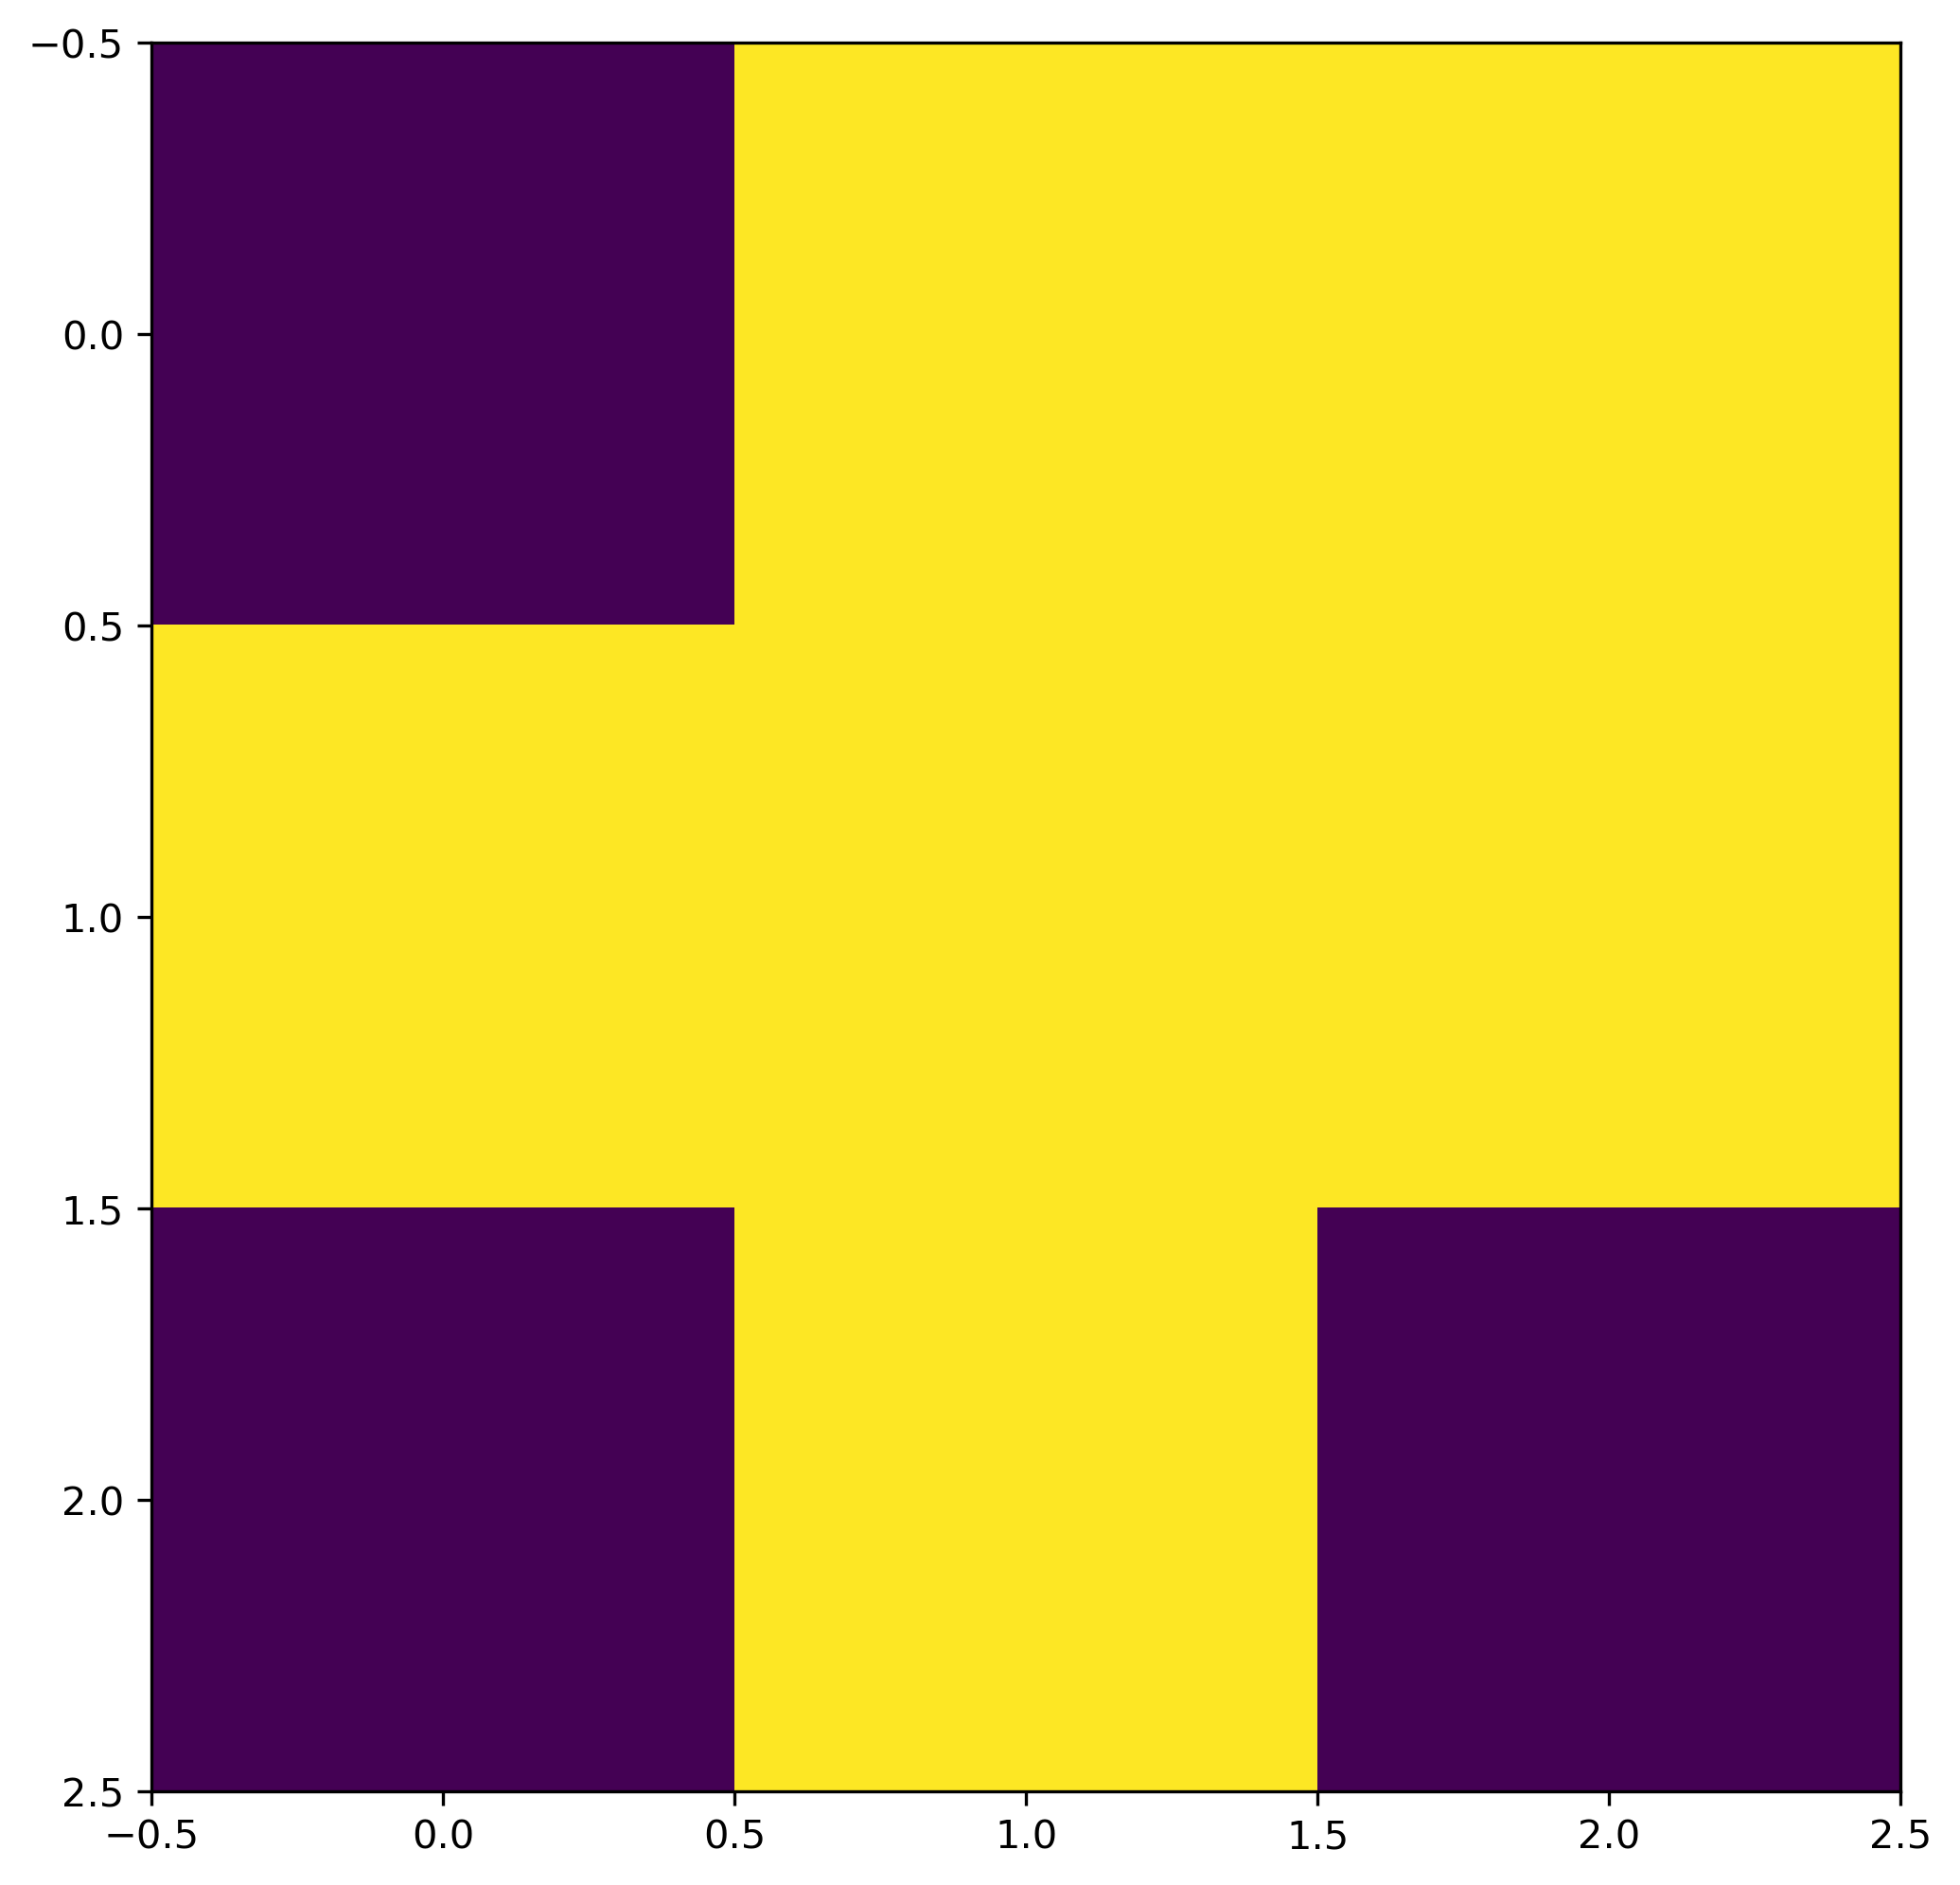
\includegraphics[width=0.4\linewidth]{images/example-s2-image.png}
  \hfill
  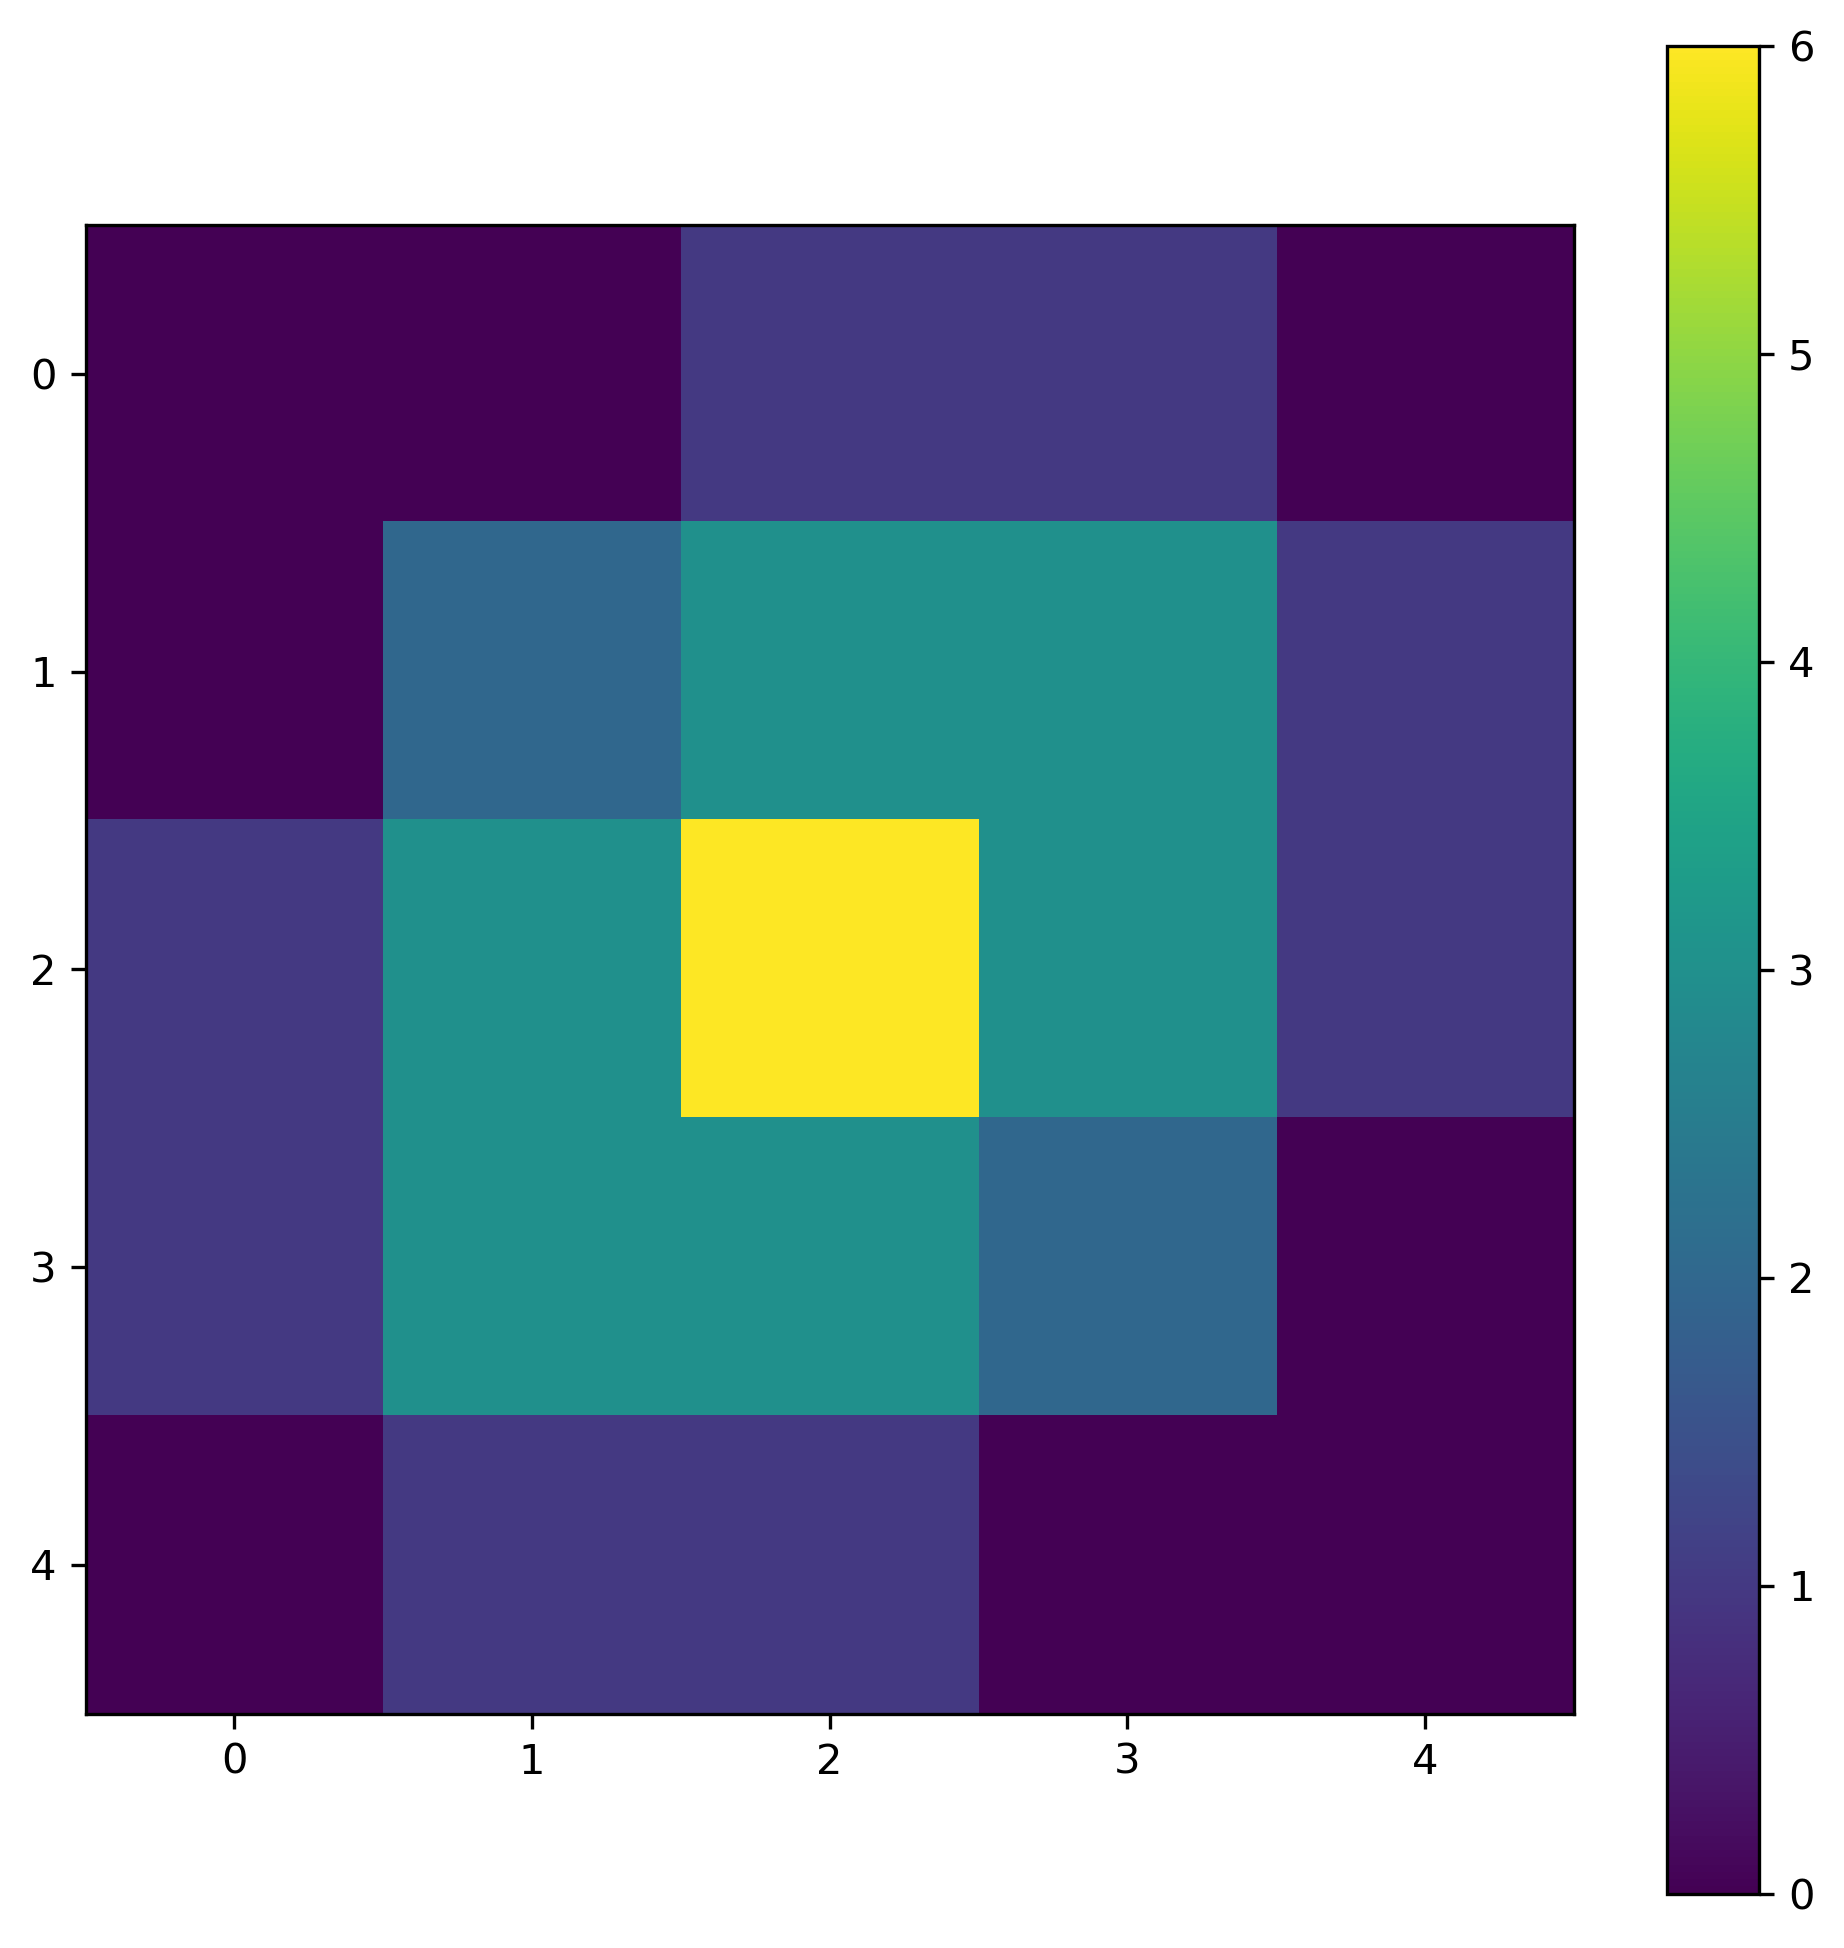
\includegraphics[width=0.4\linewidth]{images/example-s2.png}
  \caption[]{The unnormalized two-point function (right) calculated for a
    two-phase two-dimensional image (left). ``Ones'' are yellow, ``zeros'' are
    purple.}
  \label{fig:2d-example}
\end{figure*}

\subsection{Periodic boundary conditions}
Formula \ref{eq:s2z} can be applied to calculate the two-point function for a
sequence of the length $D$ under periodic boundary conditions if the calculation
if performed modulo $z^D - 1$. The group of transforms \cref{eq:group} does not
change the two-point function. This time, $S_k$ must be understood as a circular
shift by $k$ elements to the right.
\begin{example}
  Consider a sequence $(0, 1, 1, 1, 0, 1, 1)$ of length $7$. The image of its
  correlation function under Z-transform is
  $s_2(z) = 5 + 3(z+z^{-1}) + 2(z^2 + z^{-2}) + 2(z^3 + z^{-3}) + 2(z^4 +
  z^{-4}) + (z^5 + z^{-5})$.
  Taking $s_2(z) \mod x^7-1$ we obtain
  $5 + 3z + 3z^6 + 2z^2 + 2z^5 + 2z^3 + 2z^4 + 2z^4 + 2z^3 + z^5 + z^2 \mod z^7 - 1 = 5 + 3z + 3z^2 + 4z^3 + 4z^4 + 3z^5 + 3z^6$.
  The two-point correlation function is then $(5, 3, 3, 4, 4, 3, 3)$.
\end{example}

Unfortunately, there is no known way to test a sequence for non-trivial
collisions in periodic boundary conditions.

\section{Probability of encountering a polynomial with non-trivial collision.}

Suppose $f \in \mathbb{Z}[x]$ is a polynomial with independent uniformly
distributed random coefficients in $\{0, 1\}$ with the free coefficient being
equal to $1$. It is known, that the probability of $f$ being irreducible tends
to $1$ with $d = \deg f \to \infty$ \cite{konyagin1999number}.

Breuillard et~al. \cite{breuillard2019irreducibility} give the following
approximation for this probability based on extended Riemann hypothesis:
\begin{equation}
  P(\text{$f$ is irreducible}) = 1 - \sqrt{\frac{2}{\pi d}} + O(d^{-1})
  \label{eq:prob-irr}
\end{equation}

\textcolor{red}{How to cite a theorem in the paper?}
Another useful result is that for large enough $d$ the probability
of $f$ having factorization $\Phi \tilde{f}$ where $\tilde{f}$ is an irreducible
polynomial and $\Phi$ is a product of cyclotomic polynomials is at least
\begin{equation}
  p = 1 - 2\exp(-c(\log d)^{\beta - 2})
  \label{eq:prob-cyc-1}
\end{equation}
for some $c > 0$ and $\beta > 3$ if $\zeta_K$ has no zeros $\rho$ with
$|1 - \rho| < (\log d)^\alpha/d$, $\alpha > \beta$ for all $K = \mathbb{Q}(a)$
for any root $a$ of $f$.

Now we will prove a simple lemma which connects these results with collisions in
correlation functions.
\begin{theorem}
  \label{the:sequence}
  Let $A$ be a sufficiently long random sequence of 0's and 1's where each
  element is chosen randomly and independently with equal probability $1/2$ with
  exception of the first and the last elements which are 1's. Then, with
  probability at least
  \begin{equation*}
    p = 1 - 2\exp(-c(\log d)^\beta)
  \end{equation*}
  for some $c > 0$, $\beta > 1$ the sequence $A$ of the length $d+1$ does not
  have non-trivial collisions in the two-point correlation function.
\end{theorem}
\begin{proof}
  Let $f(x)$ be an image of $A$ under Z-transform and a change of variables
  $x = z^{-1}$. With probability at least $p$ it factors in $\mathbb{Z}[x]$ as
  $\Phi \tilde{f}$, where $\Phi$ is a product of cyclotomic polynomials and
  $\tilde{f}$ is irreducible. All cyclotomic polynomials with exception of
  $\Phi_1 = x - 1$ are palindromes. $\Phi_1$ does not divide $f$ because
  $f(1) = \sum\limits_{k=0}^{d-1} f_k \ge 2$. Therefore, $f$ has at most one
  non-palindrome factor and hence $A$ does not have non-trivial collisions.
\end{proof}

To obtain some results for the multidimensional case, we need to prove an
auxiliary result first.
\begin{lemma}
  \label{lem:factors}
  Let $\phi$ be a homomorphism from $R[x]$ to $R'[x]$ and $\phi f \ne const$ if
  $f \ne const$. When $f$ has no more irreducible factors (counted with their
  multiplicity) than $\phi f$.
\end{lemma}
\begin{proof}
  Suppose $f = \prod_{k=1}^n f_k^{m_k}$ where $f_k$ is irreducible in
  $R[x]$. Applying $\phi$ to $f$ we get $\phi f = \prod_{k=1}^n (\phi f_k)^{m_k}$.
  Since no $\phi f_k$ is constant, their product cannot be contracted to an
  irreducible polynomial in $R'[x]$. Each factor $\phi f_k$ can be factored to
  one or more irreducible polynomials in $R'[x]$ which proves the lemma.
\end{proof}

Now we get our main result:
\begin{theorem}
  Let $A$ be a 2-dimensional $D_1 \times D_2$ array of 0's and 1's where each
  element is chosen randomly and independently with probability $1/2$ with
  exception of two elements $A[0, 0]$ and $A[D_1 - 1, 0]$, which are 1's. Then
  $A$ does not have non-trivial collisions in the two-point correlation function
  with probability at least
  \begin{equation}
    p = 1 - \sqrt{\frac{2}{\pi (D_1 - 1)}}
    \label{eq:main-result}
  \end{equation}
\end{theorem}
\begin{proof}
  Let $f(x, y)$ be an image of $A$ under Z-transform and a change of variables
  $x = z_1^{-1}, y = z_2^{-1}$ with $\deg_x f = d$, where $d = D_1 - 1$. Let
  $\phi f = f \mod y$ be a ``partial evaluation'' homomorphism from
  $\mathbb{Z}[x, y]$ to $\mathbb{Z}[x]$. Let $f_x(x) = \phi f = f(x,0)$. Under
  conditions of the theorem $f(0) = 1$ and $\deg f_x = d$.  According to
  \cref{eq:prob-irr} we have
  \begin{equation*}
    p\{\text{$f_x$ is irreducible}\} = 1 - \sqrt{\frac{2}{\pi d}} + O(d^{-1})
  \end{equation*}
  Now we need to prove a similar result for $f$.

  We have three possible cases of factorization of $f$:
  \begin{itemize}
  \item $f$ is irreducible.
  \item $f$ factors as $f(x, y) = g(x)h(y)$. In this case
    $\phi h = h(0) = const$ and \cref{lem:factors} cannot be applied. According
    to distribution of coefficients in $f$ the probability of this case is
    $p_{split} = 2^{D_1 + D_2 - D_1 D_2 - 1}$. For any fixed integer $D_2 > 1$
    we have $p_{split} = o(D_1^{-1})$. For $D_2 = 1$ we have $f = f_x$ and
    \cref{eq:prob-irr} is applicable directly to $f$.
  \item $f$ factors as $f(x, y) = g(x, y) h(x, y)$. According to conditions on
    the coefficients $\deg_x g > 0$ and $\deg_x h > 0$, therefore
    $\phi g \ne const$ and $\phi h \ne const$. We have
    $f_x = (\phi g) (\phi h)$. Applying \cref{lem:factors}, we can say that
    $f$ is irreducible with probability at least \cref{eq:main-result}.
  \end{itemize}
  Hence $f$ is irreducible with probability at least \cref{eq:main-result}. If
  $f$ is irreducible, there is no two or more non-palindrome factors of $f$,
  hence $A$ does not have non-trivial collisions.
\end{proof}
Surely, $D_1$ can be replaced with $D_2$ in \cref{eq:main-result} if
$A[0, D_2 - 1] = 1$. This theorem also can be proved for multidimensional arrays
by recursively applying the same argument.

Despite the probability of ``meeting'' a random polynomial which has non-trivial
collisions in the two-point function is decreasing with increase of its degree,
we can easily construct ``subtrivial'' collisions of an arbitrary (sufficiently
big) degree. Let's take two polynomials $f_1, f_2$ with coefficients being in
$\{0, 1\}$. Obviously, a polynomial $f(x) = f_1(x) f_2(x^{\deg f_1 + k})$ with
integer $k > 0$ also has its coefficients in $\{0, 1\}$.

\begin{example}
  Two sequences
  \begin{align*}
    & 1101110100001101 \quad \text{and} \\
    & 1101000011011101
  \end{align*}
  are two ``subtrivial'' collisions obtained by choosing $f_1 = f_2 = 1 + x + x^3$.
\end{example}

\section{Results}
We have written a program in Common Lisp language
(\url{https://github.com/fatimp/ac-collisions-mt}) which searches for collisions
in the two-point correlation functions for random sequences of 0's and 1's with
the first and the last elements being equal to 1. The number of collisions for
each length are present in \cref{tab:numbers}. Some examples of non-trivial
collisions are in \cref{tab:collisions}.
\begin{table}[!pt]
  \centering
  \begin{tabular}{|c|c|c||c|c|c|}
    \hline
    $d$ & $N_{col}$ & $N_{irred}$ & $d$ & $N_{col}$ & $N_{irred}$\\
    \hline
    \hline
    25 & 20040 & 15146508 & 38 & 344 & 16269320 \\
    \hline
    26 & 13698 & 15400557 & 39 & 278 & 16137897 \\
    \hline
    27 & 10787 & 15241401 & 40 & 173 & 16454421 \\
    \hline
    28 & 7615 & 15656751 & 41 & 128 & 16257667 \\
    \hline
    29 & 5808 & 15365485 & 42 & 89 & 16565040 \\
    \hline
    30 & 4199 & 15883361 & 43 & 62 & 16383822 \\
    \hline
    31 & 3285 & 15595498 & 44 & 39 & 16634958 \\
    \hline
    32 & 2315 & 16023603 & 45 & 39 & 16511214 \\
    \hline
    33 & 1782 & 15821891 & 46 & 23 & 16630491 \\
    \hline
    34 & 1161 & 15988106 & 47 & 34 & 16488227 \\ 
    \hline
    35 & 926 & 15811952 & 48 & 20 & 16860506 \\
    \hline
    36 & 589 & 16356337 & 49 & 9 & 16691221 \\
    \hline
    37 & 471 & 16102018 & 50 & 13 & 16829791 \\
    \hline
  \end{tabular}
  \caption{The number of non-trivial collisions in the two-point correlation
    function and the number of irreducible polynomials for degrees
    $d = [25 \dots 50]$. The degree $d$ equals to the length of a random
    sequence minus one. The collisions were calculated by making $2 \cdot 10^7$
    random trials for each degree (polynomials were taken with repetitions).}
  \label{tab:numbers}
\end{table}
\begin{table}[!pt]
  \centering
  \begin{tabular}{|c|r|}
    \hline
    $d$ & Sequences which are non-trivial collisions \\
    \hline
    25 & 10000001000100000000100101 \\
    & 10000100010010000000000101 \\
    \hline
    & 10111111011111101111110011 \\
    & 11111011111101111110111001 \\
    \hline
    30 & 1000010000010100000000000001001 \\
    & 1000000010000010000000000101001 \\
    \hline
    & 1110111101010001100101100001111 \\
    & 1111110101001011001000111000111 \\
    & 1111010010000111000110111010111 \\
    & 1110011100001001010111010011111 \\
    \hline
    & 1110111111010101011011110111111 \\
    & 1111110111010110101011111110111 \\
    \hline
    & 1001001011011110110100110100001 \\
    & 1000010010110110110101111001001 \\
    \hline
    40 & 10010110000000000000000010011011001001011 \\
    & 11010010000000000000000011011001001101001 \\
    \hline
    & 10111111010101111111101010011111111100011 \\
    & 10010101111111101010111111011100011111111 \\
    \hline
    & 11011010010011101100011100101100110100001 \\
    & 10010010110111001000111101001100101100011 \\
    \hline
  \end{tabular}
  \caption{Examples of non-trivial collisions in the two-point correlation
    function.}
  \label{tab:collisions}
\end{table}

We have experimentally computed the probability of a sequence not having
non-trivial collisions and compared it with results of \cref{the:sequence}. The
result of comparison (taking $c = 0.148, \beta = 3.373$) is on
\cref{fig:prob-comparison}.
\begin{figure}
  \centering
  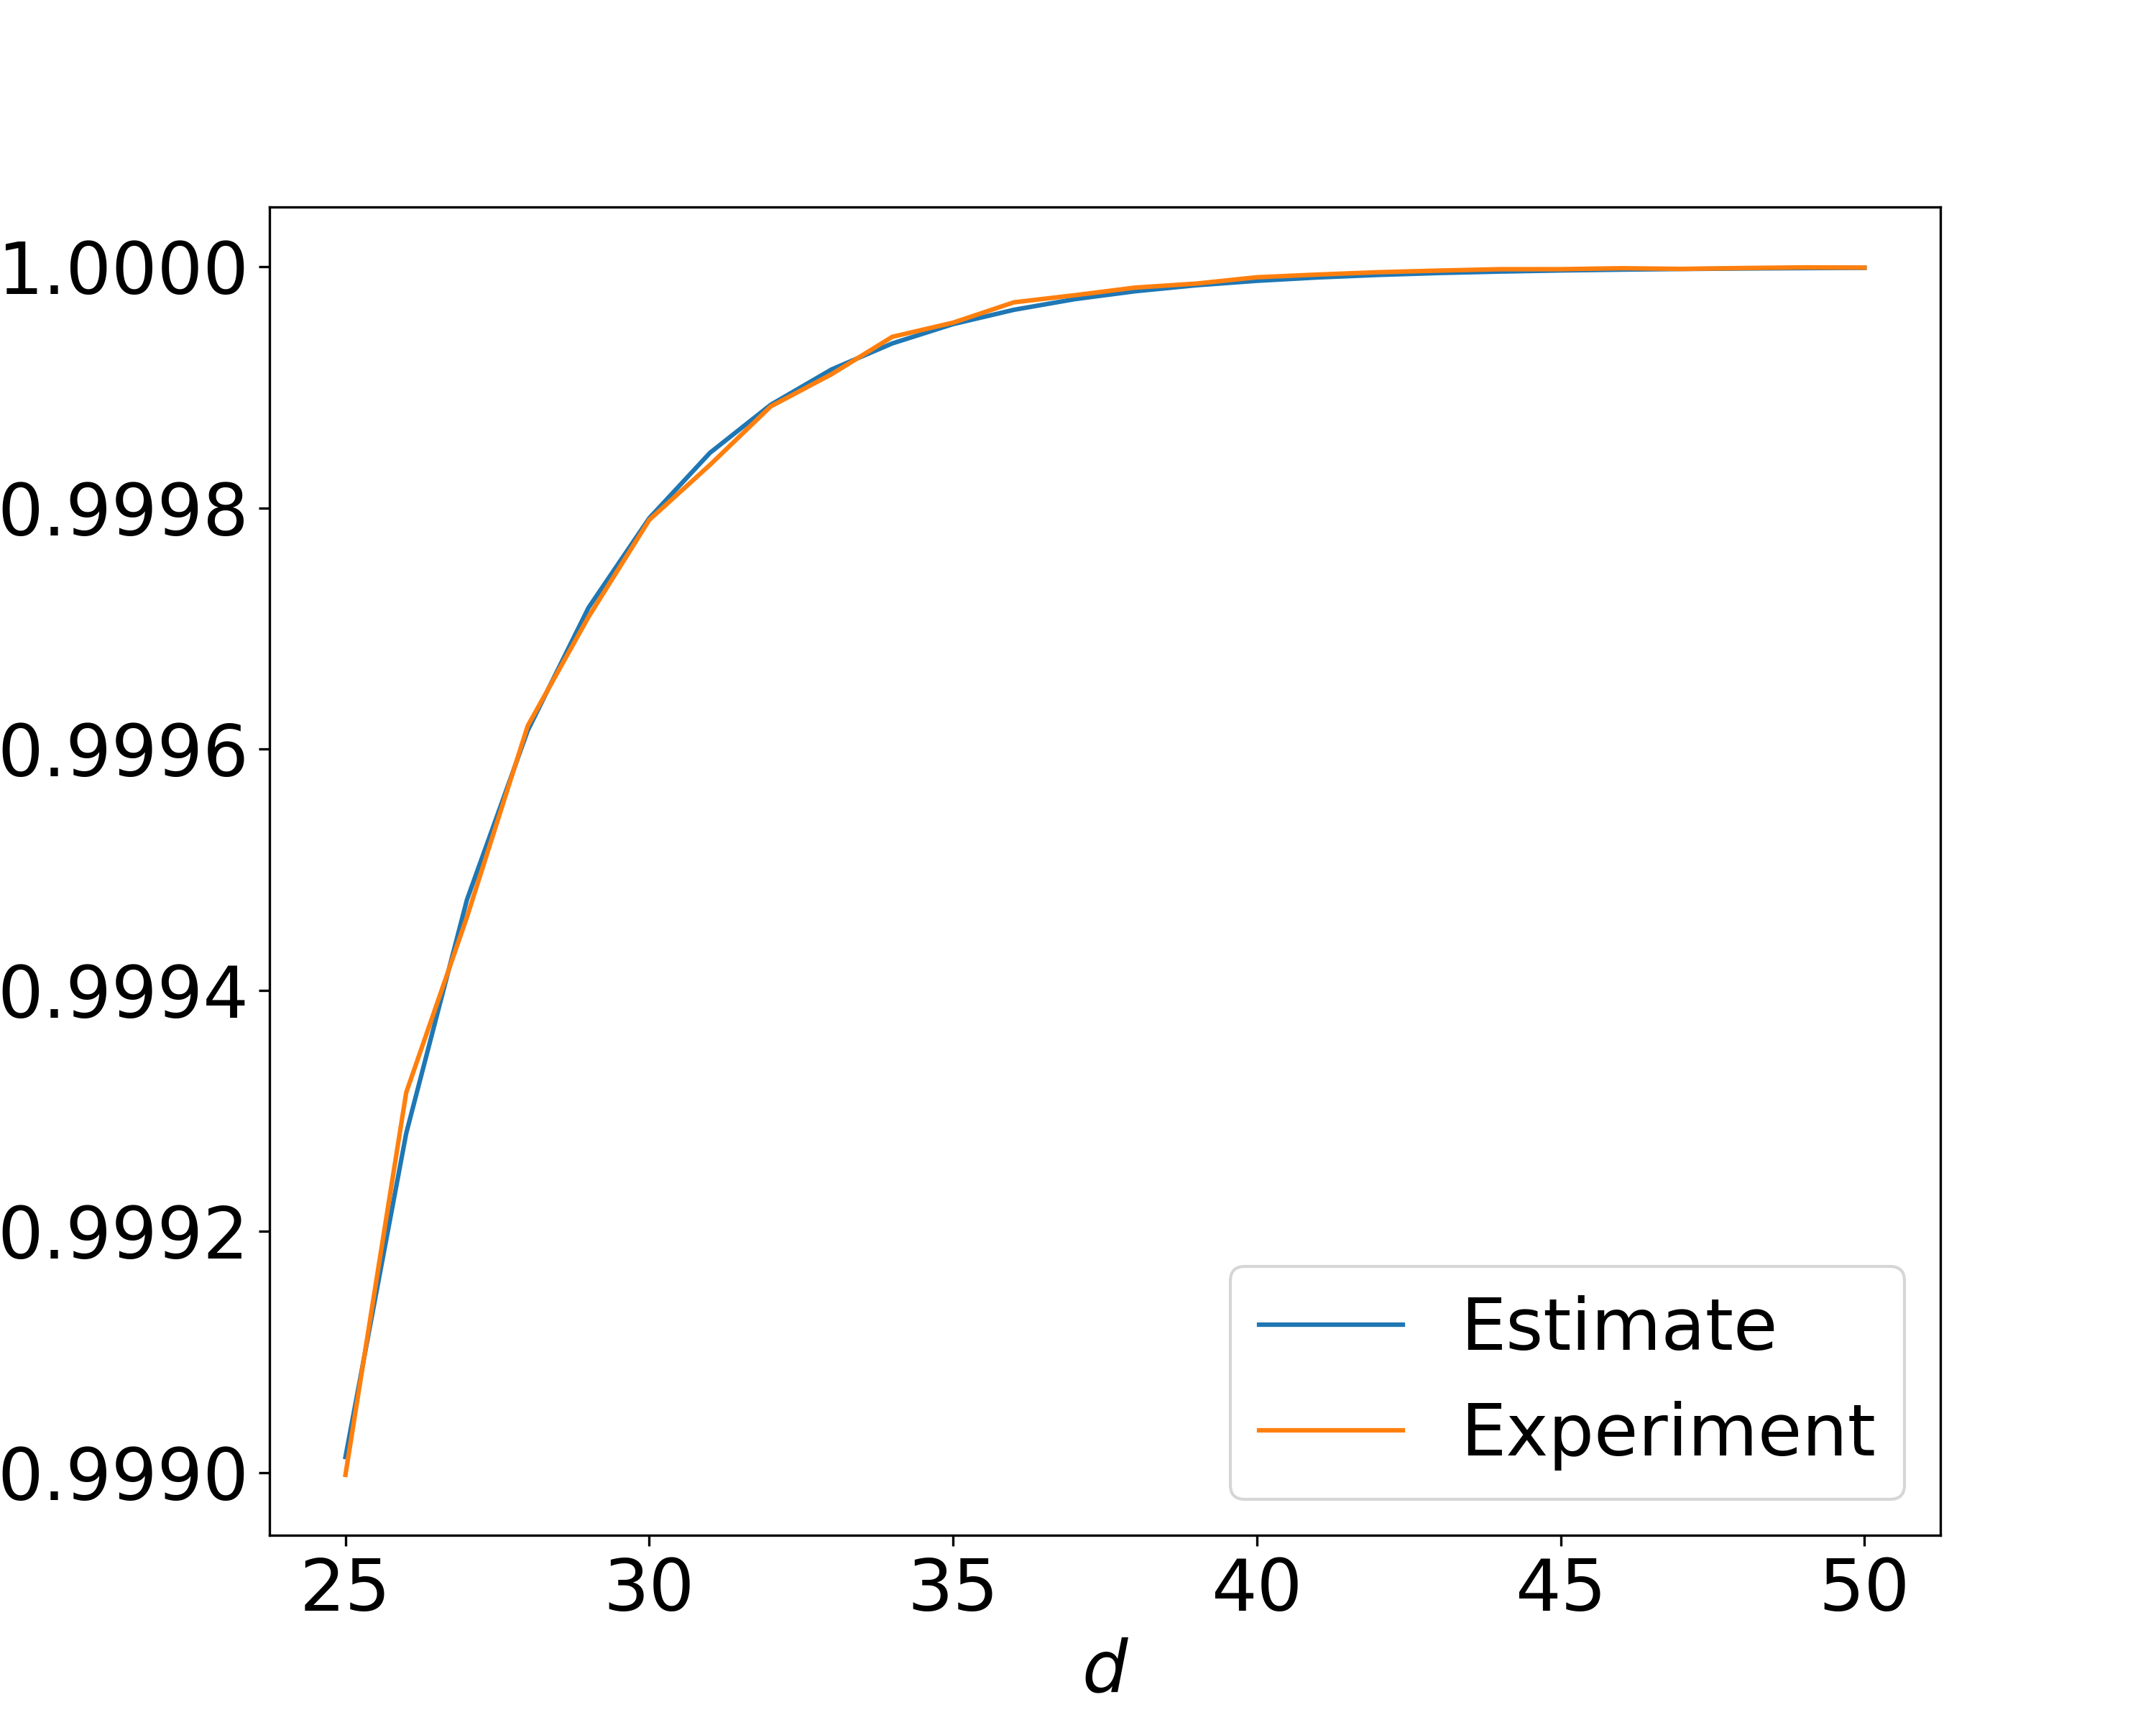
\includegraphics[width=0.5\linewidth]{images/prob.png}
  \caption[]{Probability of a sequence of 0's and 1's with length $d+1$ and the
    first and last elements being equal to 1 not to have non-trivial collisions
    in the two-point correlation function: the esimate from \cref{the:sequence}
    and a computer experiment.}
  \label{fig:prob-comparison}
\end{figure}

For two-dimensional arrays we were able to find non-trivial collisions for array
sizes at most $7 \times 7$ (with $10^6$ trials). One of such collisions is on
\cref{fig:collision-2d}.
\begin{figure*}[tp]
  \centering
  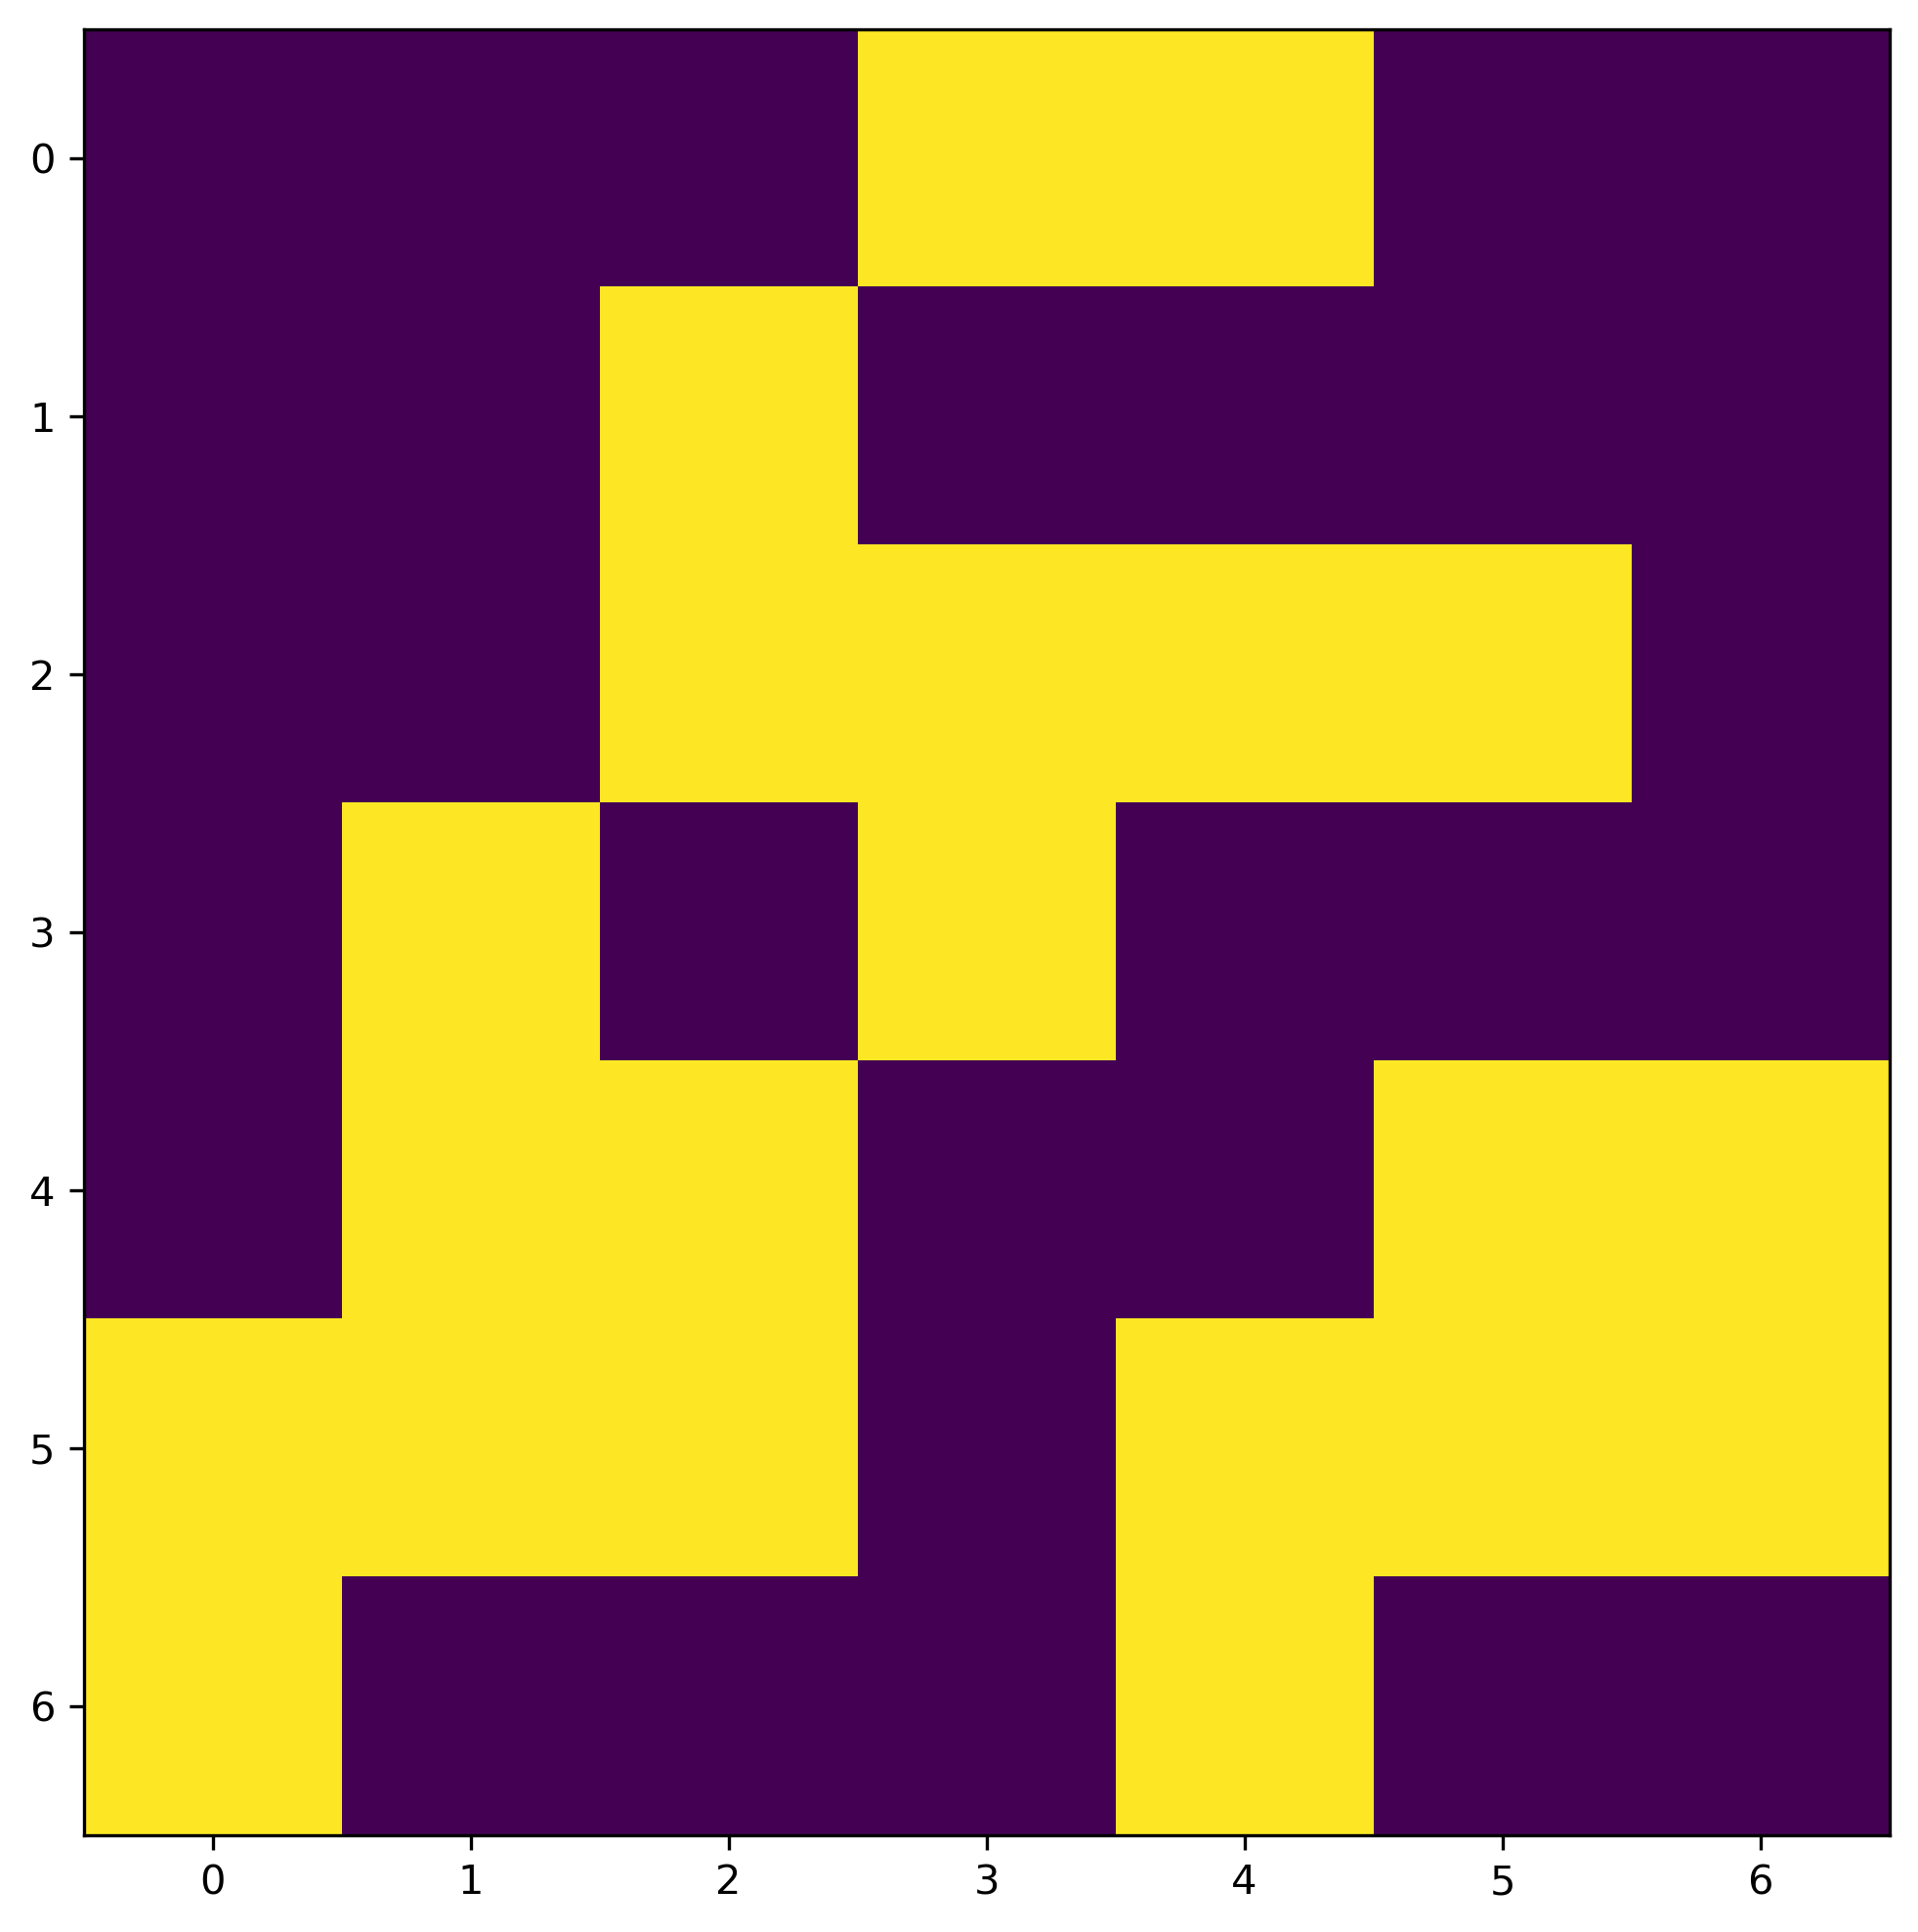
\includegraphics[width=0.3\linewidth]{images/collision-2d-1.png}
  \hfill
  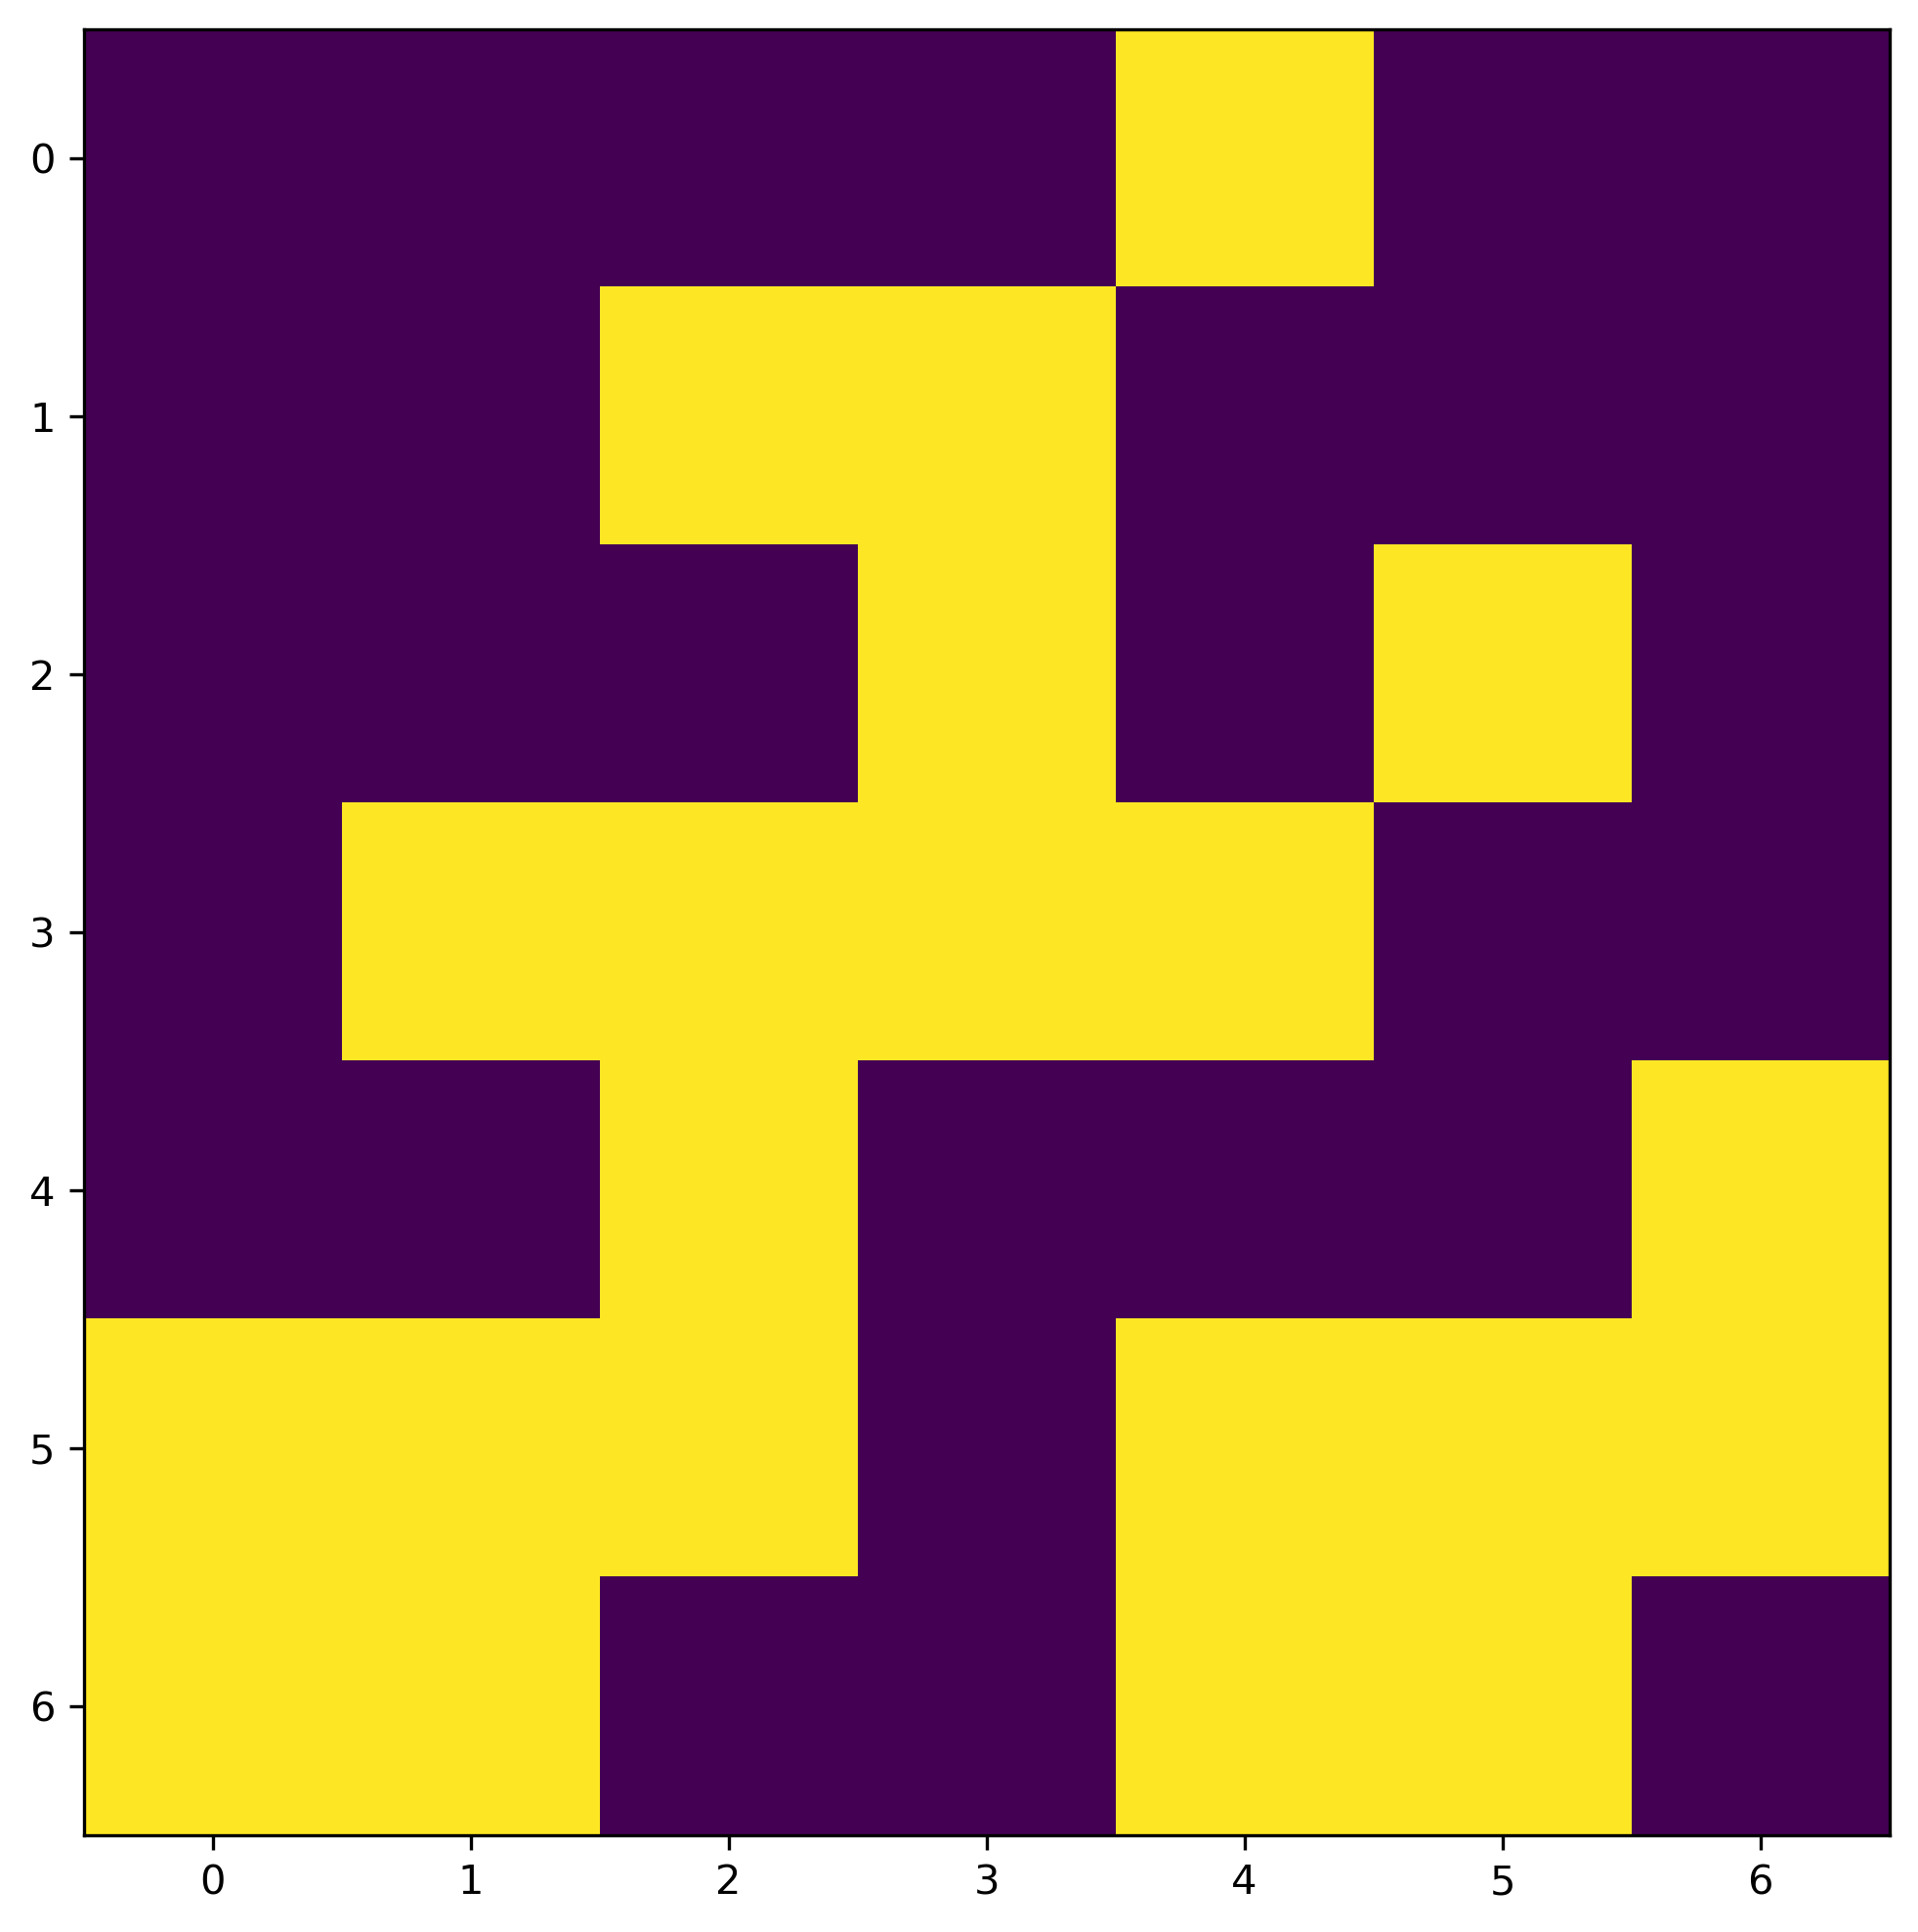
\includegraphics[width=0.3\linewidth]{images/collision-2d-2.png}
  \hfill
  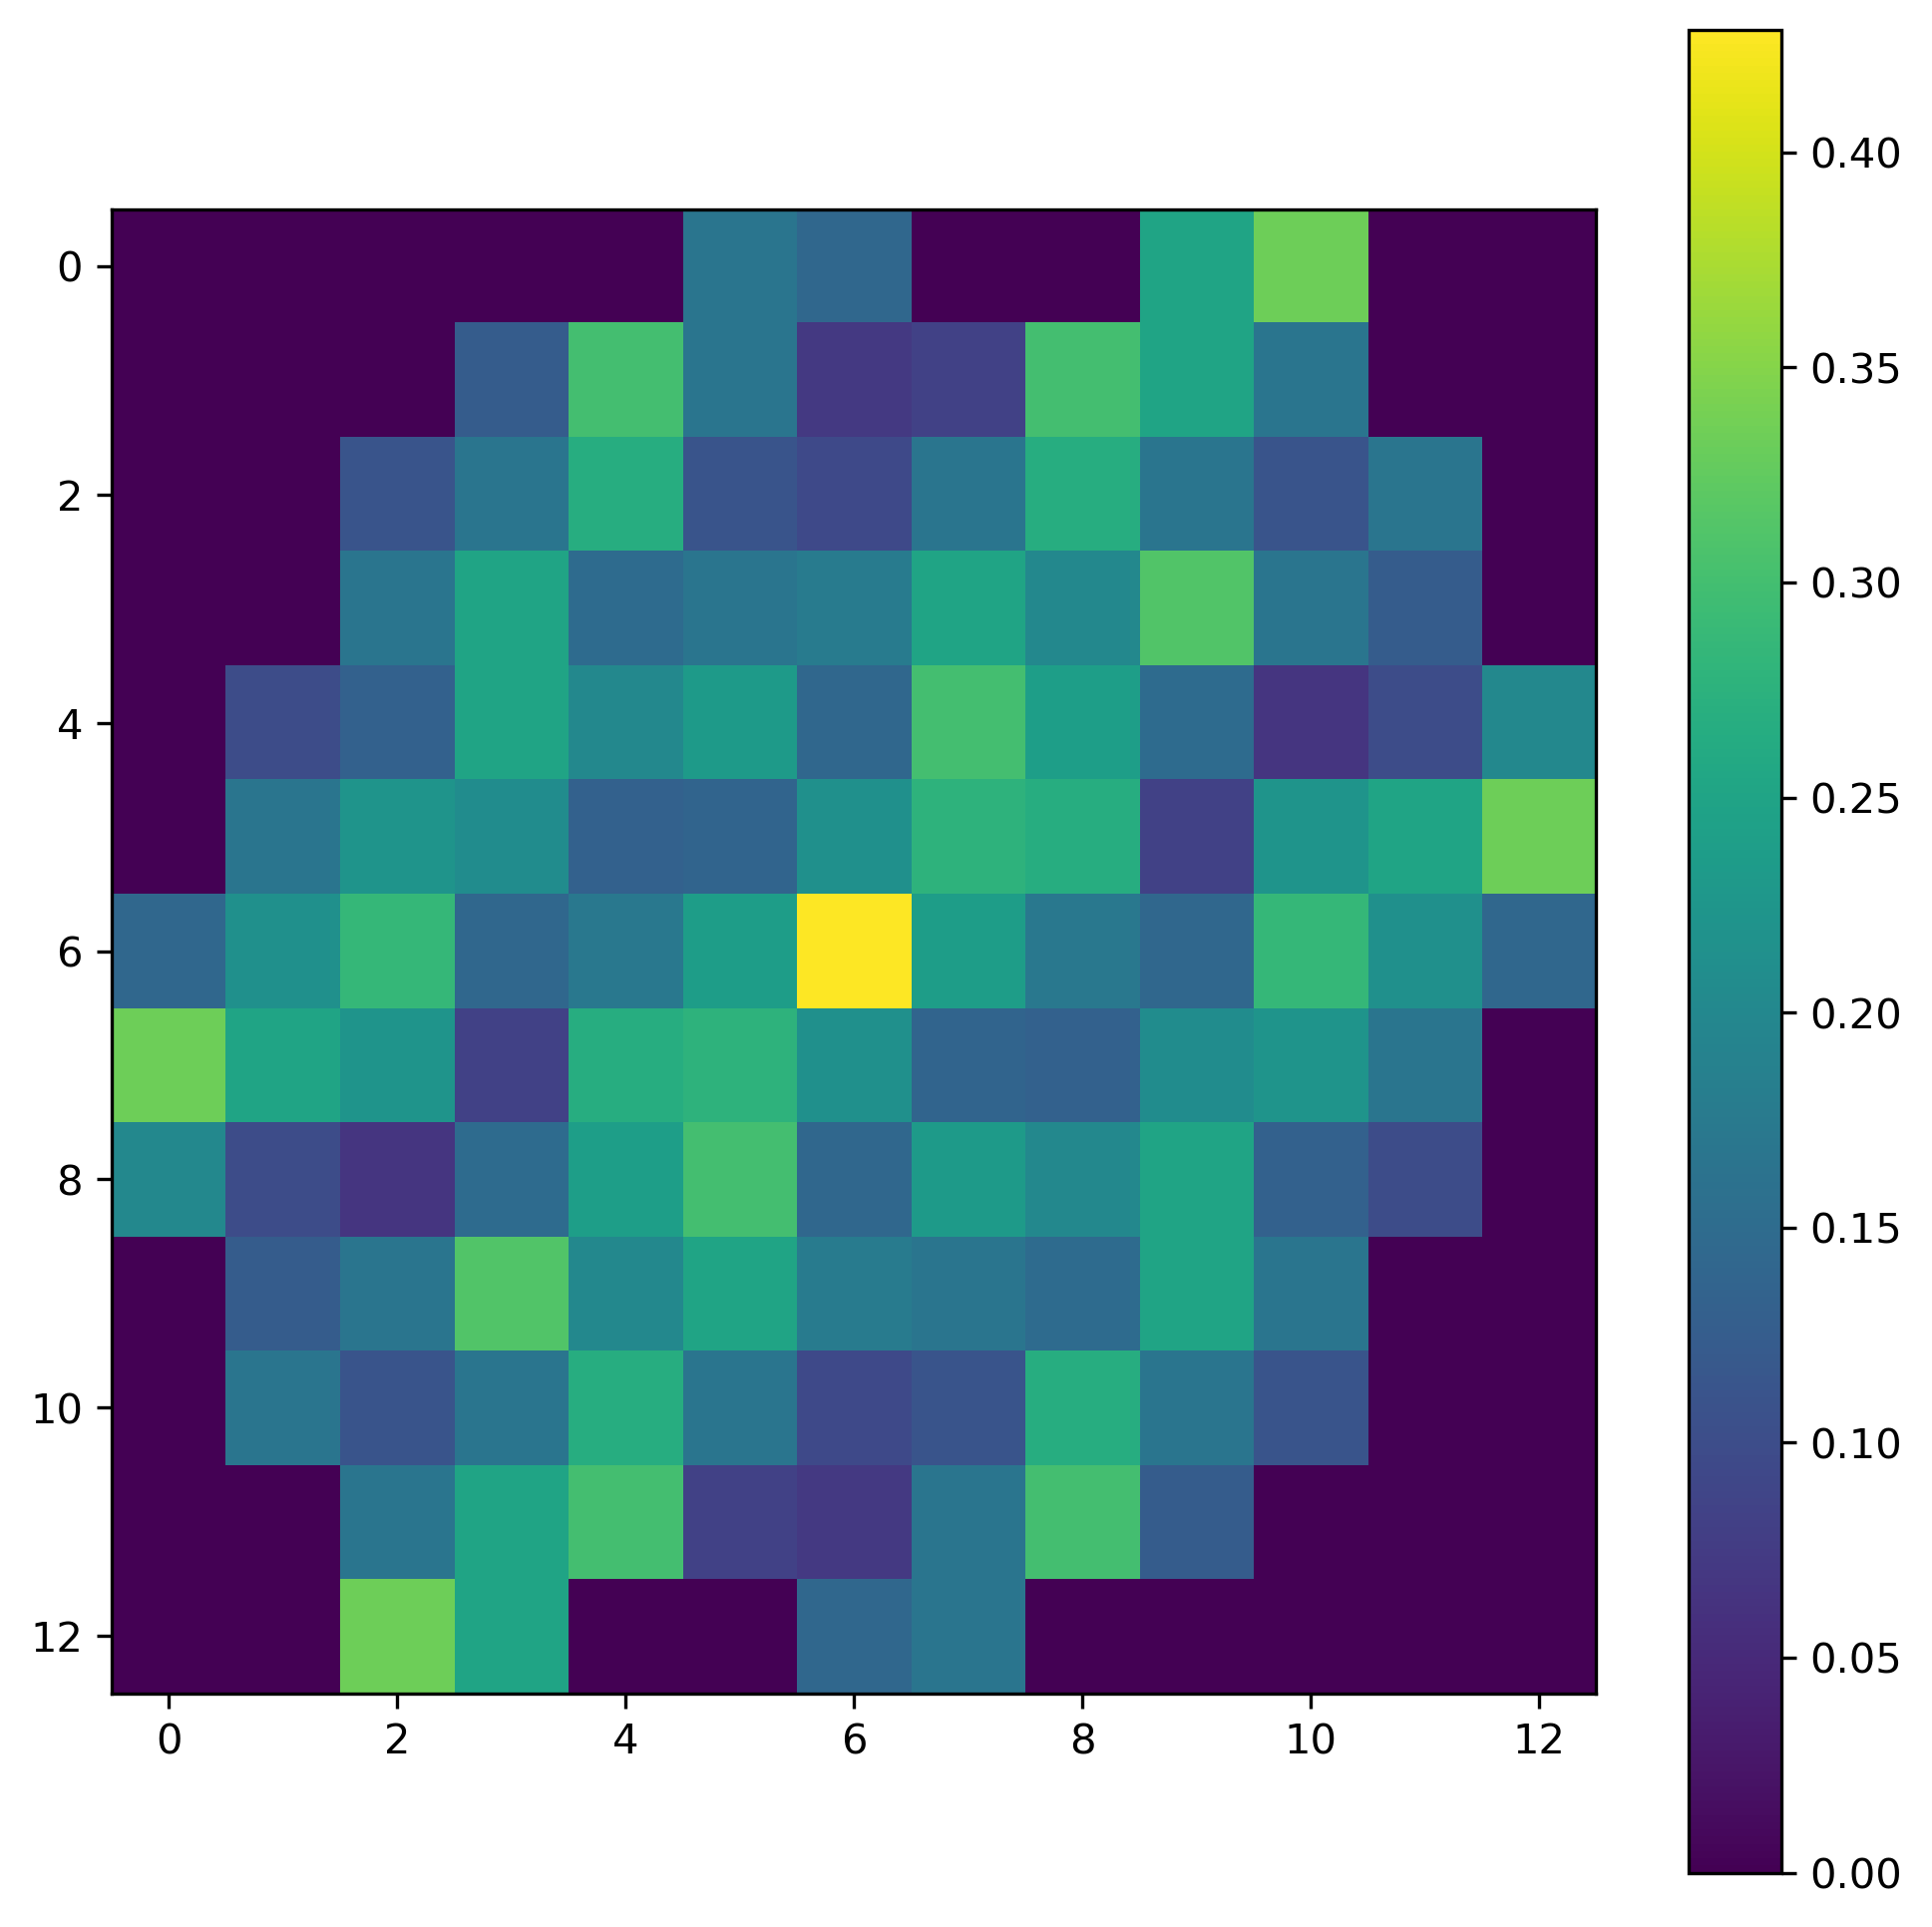
\includegraphics[width=0.3\linewidth]{images/collision-2d-s2.png}
  \caption[]{Two 2-dimensional $7 \times 7$ arrays (left, middle), having the
    same two-point correlation function (right).}
  \label{fig:collision-2d}
\end{figure*}

\newpage

\bibliographystyle{elsarticle-num}
\bibliography{paper}
\end{document}
